% ~~~~~~~~~~~~~~~~~~~~~~~~~~~~~~~~~~~~~~~~~~~~~~~~~~~~~~~~~~~~~~~~~~~~~~~~~~~~~
%
% ULL_thesis_template.tex
%
% A template for creating ULL theses which are compliant with the current
% formatting guidelines published by the Grad School.
%
% Created by: 07/17/17 - Forrest Montgomery 
%
% Modified:
%	* 05/04/18 - Daniel Newman -- danielnewman09@gmail.com
%		- Made this template compliant with Fall 2017 Graduate school guidelines
%	* 0/9/10/18 - Gerald Eaglin -- geaglin2012@gmail.com
% 		- Minor changes to match recently updated style guide
% ~~~~~~~~~~~~~~~~~~~~~~~~~~~~~~~~~~~~~~~~~~~~~~~~~~~~~~~~~~~~~~~~~~~~~~~~~~~~~
\documentclass[12pt,normalmargins]{gatech-thesis}
% Uncomment if the grad school asks you to change from Computer Modern (standard Latex font family)
% \usepackage{times}

\usepackage{amsmath,amssymb,latexsym,float,epsfig}
\usepackage{subcaption}
\usepackage{booktabs}
\usepackage{mathtools,breqn,amsmath}
\usepackage{amssymb}
\usepackage{cite}
\usepackage{bm}
\usepackage{tikz}
% \usepackage{titlesec}
\usepackage{etoolbox}
\usepackage{xcolor}

\usepackage{todonotes}
\usepackage{multirow}

\usepackage{tocloft}
\usepackage{indentfirst}
% \usepackage{etoolbox}
\definecolor{1c1}{RGB}{188,162,6}
\usepackage{ULL-style}
\usepackage[shortcuts]{extdash}

% Make sure that the caption labels are bold face
\usepackage[labelfont=bf]{caption}

% Captions inside minipages???
\usepackage[T1]{fontenc}
\usepackage[utf8]{inputenc}
\usepackage{babel}

% Rotatable Figures
\usepackage{rotating, graphicx}

% Algorithms
\usepackage{algorithm}
\usepackage{algpseudocode}

% Make the captions just the way the grad school wants them :)
% TODO: This may be able to go directly in the style file
\captionsetup[figure]{name={Figure},labelsep=period}
\captionsetup[table]{labelsep=period}


%%%%%%%%%%%%%%%%%%%%%%%%%%%%%%%%%%%
% Personal Shortcuts
% You will need to type these as \cspm{}
%%%%%%%%%%%%%%%%%%%%%%%%%%%%%%%%%%%
\newcommand{\cspm}{\textsc{cspm}}
\newcommand{\cdpm}{\textsc{cdpm}}
\newcommand{\etal}{\emph{et al.}}
%%%%%%%%%%%%%%%%%%%%%%%%%%%%%%%%%%%


%%%%%%%%%%%%%%%%
% Preliminary Info
%%%%%%%%%%%%%%%%
\title{Reinforcement Learning Based Mechanical Design \\ and Control of Flexible-Legged Jumping Robots} 
\author{Andrew Albright}
\lastnamefirstname{Albright, Andrew}

% ex: {Name}[Position] use \\ if you need a newline
% TODO: Template currently does not accept more than two readers
\committeechair{Joshua E. Vaughan}[Assistant Professor of Mechanical Engineering]
\firstreader{Alan A. Barhorst}[Department Head of Mechanical Engineering]
\secondreader{Anthony S. Maida}[Associate Professor of Computer Science]
\thirdreader{Brian Post}[Group Leader - Manufacturing Systems Design Group Oak Ridge National Laboratory]
\deanofgradschool{Mary Farmer-Kaiser}[Dean of the Graduate School]

% \major{Engineering, Mechanical Engineering Concentration}
\major{Mechanical Engineering}
\degree{Masters of Science}
\undergrad{Bachelor of Science}
\undergraduniversity{North Carolina State University}
\undergradyear{Spring 2020}
\worktype{Thesis} % or Dissertation, or Whatever

% Must be less than 300
\wordsinabstract{245}

% Total number of pages including the title page.
\totalpagesinthesis{95}
\copyrightyear{2022}

% When you graduate ex: Summer 2017
\submitdate{Spring 2022}

% \bibfiles{example-thesis}
\bibfiles{library}

\begin{document}
\iraggedright

% Change this if you want another bib style.
\bibliographystyle{gatech-thesis}
%%
\begin{preliminary}

%%%%%%%%%%%%%%%%
% Dedication -- (optional)
%%%%%%%%%%%%%%%%

% %!TEX root = ULL_thesis_template.tex 
\begin{dedication}
\vspace*{-0.35in}
\begin{center}
\vspace*{\fill}
\textit{To all the poor souls using Word, one day you will see the light that is \LaTeX.}
\vspace{\fill}
\end{center}
\end{dedication}

%%%%%%%%%%%%%%%%
% Epigraph -- A short quote suggesting the theme of the thesis,
% or something random. This is optional.
%%%%%%%%%%%%%%%%

%!TEX root = ULL_thesis_template.tex 
\begin{epigraph}

% An epigraph is a motto or quotation that captures the spirit or meaning of your work
\vspace*{-0.25in}
\begin{center}
% \vspace{-0.25in}
\vspace*{\fill}
% ``If you optimize everything, you will always be unhappy.''\\
% And the worst flaw is that we’re just plain dumb.\\
% Admit it!''\\
% --- Donald Knuth

% \textit{``Research is what I'm doing when I don't know what I'm doing.''}
% \\
% --- Wernher von Braun

% \textit{``We can lick gravity, but sometimes the paperwork is overwhelming.''}
% \\
% --- Wernher von Braun

\textit{``Before we work on artificial intelligence why don’t we do something about natural stupidity?''}
\\
--- Steve Polyak
\vspace*{\fill}
\end{center}

\end{epigraph}

%%%%%%%%%%%%%%%%
% Acknowledgements
%%%%%%%%%%%%%%%%

%!TEX root = ULL_thesis_template.tex 
\begin{acknowledgements}

I would like to firstly thank my advisor Dr. Joshua Vaughan for his leadership, both academic and personal, during my time here at the university. His support has been invaluable in helping me to understand the underlying ideas behind this material. Additionally, his constant drive to produce high quality work has kept me motivated in my attempts to do the same. I would not have completed this without him. 

I would also like to thank my committee members, Dr. Alan Barhorst, Dr. Anthony Maida and Dr. Brian Post for their input in regards to this work. Along with my lab members during my time in the C.R.A.W.LAB, Gerald Eaglin, Adam Smith, Brennan Moeller, Darcy LaFont, Thomas Poche, and Y (Eve) Dang. Their conversations and advice have greatly assisted me in my efforts to complete this work.

Lastly, I would like to thank the Louisiana Crawfish Board for their financial support, which has allowed me to work knowing my fiscal security was intact.

\end{acknowledgements}

%%%%%%%%%%%%%%%%
% Table of Contents, LOF, and LOT
%%%%%%%%%%%%%%%%
\contents
\end{preliminary}

%%%%%%%%%%%%%%%%
% Chapter 1
%%%%%%%%%%%%%%%%

%!TEX root = ULL_thesis_template.tex 
\chapter{Introduction and System Description}
\label{chapter1}
% 
\begin{figure}[b!]
  \centering
    \includegraphics[width=0.6\textwidth]{Figures/Ch1/flexible_legged_robot_fig.png}
    \caption{Flexible Robotics System}
    \label{fig:flexible_system}
\end{figure}
% 

Legged locomotive robot can have many advantages over a wheeled or tracked robots, particularly in regards to their ability to navigate uneven and unpredictable terrain \cite{Park2017,Seok2015}. They can achieve this advantage because of the numerous movement types they can deploy. Abilities such as independently placing their feet within highly rigid terrain and jumping or bounding over obstacles have been shown to be effective ways of locomoting \cite{Blackman2018}. These advantages do come at a cost, however. Legged systems are traditionally power inefficient compared to wheeled vehicles, making them a less attractive option for applications where power conservation is required. Research has shown the usefulness of adding flexible components, like the legs seen on the robot in Figure~\ref{fig:flexible_system}, for combating inefficiency and other issues \cite{Sugiyama2004,Galloway2011,Seok2015}. The addition of these components in legged robots has been shown to increase system performance measures such as running speed, jumping capability, and power efficiency \cite{Hurst2008}. However, the addition of flexible components creates a system that is highly nonlinear, and thus requires more complex control systems.  


\section{Improving Performance with Flexible Components}
%
\begin{figure}[b!]
  \centering
    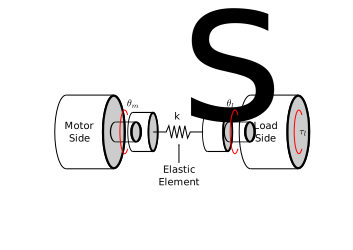
\includegraphics[width=0.7\textwidth]{Figures/Ch1/SEA.png}
    \caption{Rotary Style Series Elastic Actuator}
    \label{fig:SEA}
\end{figure}

The use of flexible components within robotic systems has been shown to be an effective way of improving performance metrics such as movement velocity and power efficiency \cite{Seok2015,Hurst2008}. Of the different techniques that have be deployed, the use of series elastic actuators (SEAs) has been shown to be effective \cite{Pratt1995,Ahmadi1997}. Storing energy in the non-rigid parts of motor joints, such as the elastic element seen in Figure~\ref{fig:SEA}, have proven to be an effective way for increasing efficiency. The addition of flexible joints is not the only technique that has been used to improve performance, however; utilizing tendon like elastic members to connect actuators to links has also been shown to be an effective way of improving efficiency \cite{Folkertsma2012}. The use of tendons, being an example of replicating what is found in nature, is a common method of finding unique mechanical designs that perform well in the real world. An example of this type of design can be seen in Figure~\ref{fig:tendon_leg}. Following a similar idea, research has also been conducted finding the usefulness of including flexibility in the spine of of 2D running robots, leading to dramatic increases in velocity \cite{Kani2013}. Research studying the effects of flexible links, like the ones shown in Figure~\ref{fig:flexible_system}, is limited though, particularly in the realm of legged-robots. Still, it has been shown as a viable method of increasing performance in these types of robots \cite{Horigomed}.
%
\begin{figure}[tb!]
  \centering
    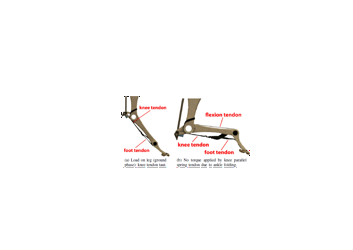
\includegraphics[width=0.75\textwidth]{Figures/Ch1/tendon_leg.png}
    \caption{Tendon Like Flexibility from \cite{Folkertsma2012}}
    \label{fig:tendon_leg}    
\end{figure}
% 

\section{Controlling Flexible Systems}
Control methods developed for flexible systems have been shown to be effective for position control and vibration reduction \cite{Luo1993, Ahmadi1997}. Due to the challenges seen in scaling the controllers to highly nonlinear systems, methods utilizing reinforcement learning are of interest. This method has been used in simple planar cases, where it was compared to a proportional-derivative (PD) control strategy for vibration suppression and proved to be a higher performing method \cite{He2020f}. Additionally, it has also been shown to be effective at defining control strategies for flexible-legged locomotion. The use of actor-critic algorithms such as Deep Deterministic Policy Gradient \cite{Lillicrap2016h} have been used to train running strategies for a flexible-legged quadruped \cite{Dwiel2019d}. Much of the research is based in simulation, however, and often the controllers are not deployed on physical systems, which leads to the question of whether or not these are useful techniques in practice. 

\section{Concurrent Design}
Defining an optimal controller for a system can be difficult due to challenges such as mechanical and electrical design limits. This is especially true when the system is flexible and the model is nonlinear. A solution to this challenge is to concurrently design a system with the controllers so that the two are jointly optimized. Defining the design process such that the design of the robot results in a simple dynamic model has been shown to improve the performance of mechatronics systems \cite{Li2001}. Additionally, in more recent work, the utilization of complex deep learning methods have shown to be an effective strategy for finding optimal concurrent designs \cite{Chen2020}. Deep learning has been used to find concurrent designs for simulated legged robotic systems, leading to improved performance in regards to movement velocity \cite{Schaff2019e}. Some research has even been completed where the designs were deployed on physical hardware, validating that this area of research is an effective one for learning how best to define system/controller architectures \cite{Whitman2020}. Little research exists utilizing these techniques on legged-robotic systems however, particularly ones with flexible components. 

\section{Reinforcement Learning}
\label{sec:rl}
With the recent successes seen in utilizing reinforcement learning (RL) to define control strategies, design parameters, and concurrent designs for robot systems, it is of interest to apply this technique in a unique way to flexible-legged jumping systems. Methods such as generative design have shown much success in being used to define mechanical designs, however most of this work is done wherein the information gathered from a system is done so in a static environment \cite{doi:10.1504/IJDE.2017.085639, briard:hal-02948764}. Reinforcement learning, in contrast, can be used to learn designs through dynamic environment interactions.

Reinforcement Learning is the process of training a policy to define a series of commands using an environment where those commands can be applied. This is an iterative process which is shown in Figure~\ref{fig:rl_process}. A policy, often referred to as an agent, from a controls theory perspective, is synonymous with a controller. The environment the controller is deployed in, again from a controls theory perspective, is synonymous with a robotic system. Training the controller requires iteratively deploying the controller's commands, or actions, to the environment and observing the results. The results are often in the form of the state of the environment and a reward resulting from the action that was applied. The reward function is defined by the designer so that the controller is trained to accomplish a desired task. Other than the reward, the controller has no way to discern what commands are good when the environment is in some state.
% 
\begin{figure}[tb!]
  \centering
    \includegraphics[width=0.5\textwidth]{Figures/Ch1/RL_Flow_Chart.drawio.png}
    \caption{Reinforcement Learning Process}
    \label{fig:rl_process}
\end{figure}
%

Learning an optimal control strategy is accomplished by deploying a gradient-decent-based learning algorithm utilizing information such as the state of the environment and the reward. For general robotics applications, at each discrete time step $t$, the environment will be in a state $s \in \mathcal{S}$, and the controller will select an action $a \in \mathcal{A}$ according to the current policy $\pi~:~\mathcal{S}~\rightarrow~\mathcal{A}$ and apply said action within the environment. The environment will transition to a new state $s'$ and will generate a reward $r$ based on the designer's definition of the reward function. The return, being the value the algorithm is trying to optimize, is defined as a discounted sum of rewards, $R_t = \sum_{i=t}^T \gamma^{i-t} \, r(s_i, a_i)$, where $\gamma$ is a discount factor for assigning the level of importance for near-term or long-term rewards.

The challenge of an RL algorithm is to optimize a policy, $\pi_{\phi}$, with parameters, $\phi$, such that actions generated at each time step will maximize the return. Ultimately, an optimized policy will maximize the expected return, $J(\phi) = \mathbb{E}_{s_i \thicksim p_{\pi}, a_i \thicksim \pi}[R_0]$. 
% Because many robotics controls processes are continuous control problems, the policy, $\pi_{\phi}$, can be updated using gradient decent in terms of the parameters $\phi$, which looks like $\nabla_{\phi} J(\phi)$. 

\section{Twin Delayed Deep Deterministic Policy Gradient}

There are many algorithms used to train a neural-network-based controller in an RL application, some of which have shown their ability to learn high-performing control strategies for robotic systems \cite{Zhao2020, Vecerik2017, Plappert2018}. Of the different algorithms used in current research, the one selected and tested in this work is Twin Delayed Deep Deterministic Policy Gradient (TD3) \cite{Fujimoto2018d}. This is an actor-critic learning algorithm which is widely considered the successor to the popular and proven Deep Deterministic Policy Gradient (DDPG) algorithm \cite{Lillicrap2016h}. 

\begin{sidewaysfigure}
  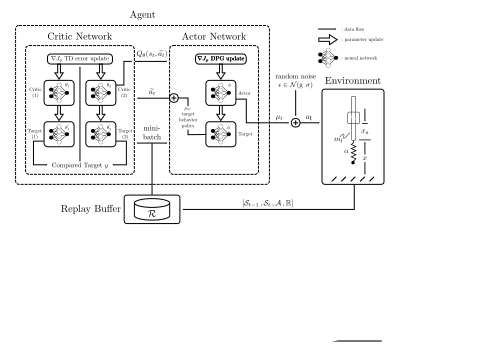
\includegraphics[width=\textwidth]{Figures/Ch1/TD3_Diagram.png}
  \caption{Twin Delayed Deep Deterministic Policy Gradient Block Diagram with Monopode as Environment}
  \label{fig:TD3}
\end{sidewaysfigure}

Figure~\ref{fig:TD3} displays the flow of information for this algorithm. In general, this algorithm learns both a Q-function and a policy, being the \textit{critic} and the \textit{actor}. For algorithms such as TD3, the ultimate goal is to find a policy, $\pi_{\theta}$, which maximizes the expected return:
% 
\begin{equation}
  \label{eq:expected_return}
  \begin{aligned}
    \nabla_{\phi} J(\phi) = \mathbb{E}_{s \thicksim p_{\pi}} \left [ \nabla_a Q^{\pi}(s,a)|_{a=\pi(s)} \nabla_{\phi}\pi_{\phi}(s) \right ]
  \end{aligned}
\end{equation}
%
where $Q^{\pi}(s,a) = \mathbb{E}_{s_i \thicksim p_{\pi}, a_i \thicksim \pi}[R_t|s,a]$ is the Q-function (sometimes called the value function) and the critic in the case of the TD3 architecture. This function is based on the Bellman Equation \cite{BellmanEquation} and returns a numerical value from being in a state $s$, taking action $a$, and following policy $\pi$ from there after:
% 
\begin{equation}
  \label{eq:bellman_eq}
  \begin{aligned}
    Q^{\pi}(s,a) = \underset{s' \thicksim P}{E} \left[ r(s,a) + \gamma \, \underset{a'}{\textup{max}} \, Q^{\pi}(s', a')  \right]
  \end{aligned}
\end{equation}
% 

Using a differentiable function approximator, $Q^{\pi}(s,a)$ can be represented and estimated by $Q_{\phi}(s,a)$, with parameters $\phi$ \cite{Mnihg}. Updating the Q-function is accomplished using the temporal difference error between the Q-function and a target Q-function \cite{Sutton1991, Watkins1989}. To maintain a fixed objective over multiple policy updates, the target Q-function approximator is instantiated separately as $Q_{\phi_{targ}}(s,a)$. The target does depend on the same parameters that are being trained, $\phi$, so there exists an issue when trying to use it as a target. To solve this issue the target network is updated at a delayed pace following the main Q-function approximator by either matching the parameters or by polyak averaging, $\phi_{targ} \leftarrow \tau \phi + (1-\tau)\phi_{targ}$, where $\tau$ is a tunable hyperparameter. 

In summary, the critic side of the TD3 algorithm is responsible for minimizing the difference between the value of the current state/action pair using the main Q-function, and the reward of the current state/action pair plus the discounted value of the next state/action pair using the target Q-function. The loss function takes the form:
% 
\begin{equation}
  \label{eq:q_func_loss}
  \begin{aligned}
    L(\phi, \mathcal{D}) = \underset{(s,a,r,s',d) \thicksim \mathcal{D}}{E} \left[ \left( Q_{\phi}(s,a) - \left( r(s,a) + \gamma \, (1-d) \, Q_{\phi_{targ}}(s', \pi_{\theta_{targ}}(s')) \right)  \right)^2 \right]
  \end{aligned}
\end{equation}
% 
where $\pi_{\theta_{targ}}(s')$ is a target policy that, in a similar manner to the target Q-function, follows the main policy, $\pi_{\theta}$, at a delayed pace either by directly copying the values or by Polyak averaging. Additionally, $d$ represents a boolean value which depends on the terminal status of the next state, $s'$. 

As for updating the policy for the actor critic-type algorithm, this aspect is rather simple. Because DDPG, and therefore TD3, are built to accommodate only continuous action spaces, the Q-function is assumed to be differentiable with respect to action. Therefore, to find optimal policy parameters, $\theta$, for the policy, $\pi_{\theta}$, the solution of the Q function must be found:
% 
\begin{equation}
  \label{eq:policy_update}
  \begin{aligned}
    \underset{\theta}{\textup{max}} \, \underset{s \thicksim \mathcal{D}}{E} \, \left[Q_{\phi}(s, \pi_{\theta}(s))\right]
  \end{aligned}
\end{equation}

The reason that TD3 is considered the successor to DDPG is that there are some additional tricks deployed in addition to the description thus far. The first is the addition of noise to the target policy. It can be seen in~(\ref{eq:q_func_loss}) that the target policy, $\pi_{\theta_{targ}}$, is required to generate an action to evaluate the target Q-function. Noise is added to the policy, taking the form:
% 
\begin{equation}
  \label{eq:action_noise}
  \begin{aligned}
    a'(s') = \textup{clip} \, \left( \pi_{\theta_{targ}}(s') + \textup{clip}(\epsilon, -c, c), a_{low}, a_{high}  \right), ~~~ \epsilon \thicksim \mathcal{N}(0,\sigma)
  \end{aligned}
\end{equation}
% 
where $\epsilon$ represents the noise sampled using some user specified method. This method of adding noise was shown to reduce the issue of the Q-function approximator developing large values for certain state/action pairs, therefore smoothing the Q-function. 

The second trick the TD3 algorithm employs is the addition of a second Q-function approximator and target Q-function approximator. A known potential issue of the Q-function is that it can suffer from overestimation of the value of action/state pairs. This, of course, leads to the policy learning actions that the Q-function assumes are better than they actually are. To alleviate this issue, two Q-functions and two target Q-functions are instantiated. Calculating the target Q-function is then completed by evaluating the two target Q-functions:
% 
\begin{equation}
  \begin{aligned}
    y(r,s',d) = r(s,a) + \gamma \, (1-d) \, Q_{\phi_{i,targ}}(s', \pi_{\theta_{targ}}(s')),~~~ \textup{for}~i=1,2
  \end{aligned}
\end{equation}
% 
and taking the lower of the two targets to update both the main Q-functions:
% 
\begin{equation}
  \begin{aligned}
    L(\phi_1, \mathcal{D}) = \underset{(s,a,r,s',d) \thicksim \mathcal{D}}{E} \left[ \left( Q_{\phi_1}(s,a) - y(r,s',d) \right)^2 \right]
  \end{aligned}
\end{equation}
% 
\begin{equation}
  \begin{aligned}
    L(\phi_2, \mathcal{D}) = \underset{(s,a,r,s',d) \thicksim \mathcal{D}}{E} \left[ \left( Q_{\phi_2}(s,a) - y(r,s',d) \right)^2 \right]
  \end{aligned}
\end{equation}.
% 

The last technique that the TD3 algorithm employs is the addition of a delay between to the policy update in regards to the Q-function update. It has been shown that in doing this the Q-function is able to converge to a better solution before updating the policy. Ultimately, the addition of a policy update delay was utilized to reduce coupling between the Q-function and the policy. The recommended delay is updating the policy every two Q-function updates.

There are many implementations of the TD3 algorithm that are publicly available. Of these, the \textbf{\textbf{StableBaselines3}} implementation is used to complete the work in this thesis \cite{stable-baselines3}. \textbf{\textbf{StableBaselines3}} is a widely used library of RL algorithm implementations and is composed of well written and understandable documentation for the supported implementations. The differentiable function approximators used to estimate the policies and Q-functions are built within \textbf{StableBaselines3} using PyTorch \cite{NEURIPS2019_9015}, which is also a widely used framework for machine learning and more specifically reinforcement learning. 

\section{Contributions}

The purpose of the work presented in the remainder of this thesis is to propose and evaluate the performance of a concurrent design architecture that utilizes RL techniques for flexible jumping systems. A concurrent design system in this work is one that concurrently learns a mechanical/electrical design for a system and an associated control policy for said system. There is an absence of literature surrounding RL-based concurrent design, particularly regarding locomotive robotics applications. Therefore, in this work, an RL-based method is proposed that seeks to learn better performing designs than ones that implement isolated mechanical/electrical and controller policy design. The method will be evaluated in simulation on a simplified flexible-legged jumping monopode where better designs are ones that jump higher and perform more efficiently. The components which build the concurrent design architecture will be split across the next few chapters wherein additional findings will be presented.

In the next chapter, a RL-based controller will be trained on a monopode jumping system to evaluate the effectiveness of training for efficient control. Power use is often considered when designing RL controllers for rigid systems, typically taking the form of a weighted negative reward when deploying an RL algorithm. It will be evaluated by defining strategies for flexible systems, where efficiency is the primary objective, if the resulting control strategy takes advantage of system flexibility. To determine if the learned policies are approaching what current literature supports regarding optimal control, the performance will be evaluated against input shaping techniques in Chapter~\ref{chapter3}.

Additionally, the need arises for incorporating mechanical design parameters into the learning process. Therefore, in Chapter~\ref{chapter4}, an RL problem is defined in a unique way such that the environment the RL policy is deployed in is a simulation of an environment where the actions sent by the policy are mechanical design updates. The method will be evaluated on the monopode jumping system to learn mechanical design parameters related to flexibility. Futhermore, using a single, fixed control input, it is of interest to determine if this technique can be used to define designs to accomplish multiple tasks. Therefore, using a single control input generated from the aforementioned input shaping techniques, the RL learning method will be tested for learning designs that cause the monopode to jump to multiple heights.

Next, in Chapter~\ref{chapter5}, the methods of learning a control policy and a design will be combined to create a concurrent design architecture. Two methods of implementing the mechanical design update will be shown, and the effects of the two methods will be discussed. Furthermore, a newly introduced hyperparameter when implementing the constructed concurrent design will be evaluated and the results will be discussed. The methods will be tested to compare efficient jumping and non-efficient jumping concurrent designs for the monopode jumping system. Ultimately, the resulting concurrent design performance will be presented and compared to the performance of control policies trained on static designs.

Lastly, in Chapter~\ref{chapter6}, the work presented in this thesis will be summarized and the results of the proposed concurrent design process will be highlighted. Accompanying the conclusive remarks, future research that has been enabled by the work presented will be discussed, along with recommended next steps for starting this future work.  
%%%%%%%%%%%%%%%%
% Chapter 2
%%%%%%%%%%%%%%%%

%!TEX root = ULL_thesis_template.tex 
\chapter{Learning Efficient Jumping Strategies for the Monopode System}
\label{chapter2}

% \section{Learning Control Strategies}

Utilizing reinforcement learning to train a neural network based controller has been shown to be useful for controlling many robotic systems \cite{Vecerik2017, Plappert2018}. It has been used to successfully control rigid-legged robots both in simulation and on physical hardware \cite{Ha2020a, Zhao2020}. Reinforcement learning has been shown to be capable of defining more effective and efficient-jumping techniques for a single-legged robot with SEAs \cite{Fankhauser2013}. It has also been shown to be an effective method for controlling multi-legged robots both in simulation and on physical hardware \cite{Xiao2019, Haarnoja2019a, Tsounis2019}. Furthermore, it has been shown to be useful for defining energy efficient strategies for multi-legged robots that have been deployed on physical hardware \cite{Da2020c}. However, the body of work demonstrating the use of RL to train controllers for flexible systems is limited, particularly in regards to legged locomotive systems. In this chapter, RL is deployed to define an energy efficient-jumping strategy for a monopode jumping system. The purpose of this work is to validate the use of RL for defining the control aspect of a concurrent design architecture for flexible jumping systems.

\section{Monopode Jumping System}
\label{sec:monopode}
To evaluate the methods discussed in this chapter, a monopode system like the one shown in Figure~\ref{fig:monopode} was used to represent a flexible jumping system. This system has been studied and has been shown to be an effective base for modeling the jumping gaits for many different animals \cite{Blickhan1993a}.

\begin{figure}[tb!]
    \centering
      \includegraphics[width=0.25\textwidth]{Figures/Ch1/monoped.png}
      \caption{Monopode Jumping System}
      \label{fig:monopode}
\end{figure}
% 

The monopode is controlled by accelerating the actuator mass, $m_a$, along the rod mass, $m_l$, causing a hopping-like motion. The system contacts the ground through a nonlinear spring, represented by the variable $\alpha$ in the figure. Also included in the model is a damper parallel with the spring, having a damping coefficient of $c$, though it is not shown in the figure. Variables $x$ and $x_a$ represent the global position of the rod and the local position of the actuator with respect to the rod, respectively. The equation of motion for the system is: 
% 
\begin{equation}
    \label{eq:eom}
    \begin{aligned}
        \ddot{x} = \frac{\gamma}{m_t} \left(\alpha\,x + \beta\,x^3 + c\,\dot{x}\right)-\frac{m_a}{m_t}\,\ddot{x}_a-g 
    \end{aligned}
\end{equation}
%
where $x$ and $\dot{x}$ are position and velocity of the rod, respectively, the acceleration of the actuator, $\ddot{x}_a$, is the control input, and $m_a$ and $m_t$ are the mass of the actuator and the complete system, respectively. Constants $\alpha$ and $c$ represent the nonlinear spring and damping coefficient, respectively, and constant $\beta$ is set to $1e8$. Ground contact determines the value of $\gamma$, so that the spring and damper do not apply any force while the leg is airborne:
% 
\begin{equation}
    \label{eq:gamaa}
    \gamma =
    \left\{\begin{matrix}
        -1, & x \leq 0\\ 
        \hphantom{-} 0, & \mbox{otherwise}
    \end{matrix}\right.
\end{equation}  
% 
Additionally, the spring compression limit, or the systems position in the negative $x$ direction, is limited to 0.008m. The system is also confined to move only vertically so that controlling balance is not required. The values of the parameters shown in Figure~\ref{fig:monopode} are displayed in Table~\ref{tab:monopode_params}. 
% 
\begin{table}[tb!]
  \caption{Monopode Model Parameters}
    \begin{center}
    \vspace{-12pt}
      \begin{tabular}{c c}
        \textbf{Model Parameter}                                 & \textbf{Value}                                    \\
        \hline
        \hline
        Mass of Leg, $m_l$                                       & 0.175 kg                                          \\
        Mass of Actuator, $m_a$                                  & 1.003 kg                                          \\
        Spring Constant, $\alpha_{nominal}$                      & 5760 $\textup{N}/\textup{m}$                      \\
        Natural Frequency, $\omega_n$                            & $\sqrt{\frac{\alpha}{m_l + m_a}}$                 \\
        Damping Ratio, $\zeta_{nominal}$                         & 1e-2 $\frac{\textup{N}}{\textup{m/s}}$            \\
        Gravity, $g$                                             & 9.81 m/s$^2$                                      \\
        \hline
        Actuator Stroke, $(x_{a})_{\textup{max}}$                & 0.008 $\textup{m}$                                \\
        Max.\ Actuator Velocity, $(\dot{x}_{a})_{\textup{max}}$  & 1.0 $\textup{m}/\textup{s}$                       \\ 
        Max.\ Actuator Acceleration, $(\ddot{x}_{a})_{\textup{max}}$   & 10.0 $\textup{m}/\textup{s}^2$              \\
        \hline
        \hline
      \end{tabular}
      \label{tab:monopode_params}
      % \vspace{-12pt}
    \end{center}
\end{table}
%  

\section{Training Environment}
Using the monopode model, an environment aligning with the standards set by OpenAI for a Gym environment was created \cite{Brockman2016c}. The observation and action spaces were defined, respectively, as follows:
% 
\begin{equation}
  \mathcal{S} = \left[ x_{a_t}, \dot{x}_{a_t}, x_t, \dot{x}_t \right]
\end{equation}
% 
\begin{equation}
  \mathcal{A} = [\ddot{x}_{a_t}]
\end{equation}
% 
where $x_t$ and $\dot{x}_t$ were the monopode's position and velocity at time $t$, and $x_{a_t}$, $\dot{x}_{a_t}$ and $\ddot{x}_{a_t}$ were the actuator's position, velocity and acceleration, respectively.

Two separate stopping conditions were defined for the environment to evaluate two different jump types and therefore two different jumping commands. The first was defined as the position of the monopode being greater than zero then returning to zero once. The second condition was defined like the first condition, but with the position of the monopode being greater than zero and then returning than zero twice.

Two different jumps were created from these stopping conditions. The first was a single jump command, and the second a stutter jump command. The intent of utilizing two different jumping commands was to determine if an RL algorithm was more or less effective in learning differing strategies depending on the complexity of the desired command. 

% 
\begin{figure}[tb!]
  \centering
  \begin{subfigure}{.75\textwidth}
    \centering
    \includegraphics[width=\linewidth]{Figures/Ch2/single_jump.png}
    \caption{Example Single Jump}
    \label{fig:singleJump}
  \end{subfigure} \\
  \begin{subfigure}{.9\textwidth}
    \centering
    \includegraphics[width=\linewidth]{Figures/Ch2/stutter_jump.png}
     \caption{Example Stutter Jump}
     \label{fig:stutterJump}
  \end{subfigure}
   \caption{Jumping Types for the Monopode Jumping System}
   \label{fig:jump_types}
\end{figure} 

An example single jump is shown in Figure~\ref{fig:singleJump}. The intended command from the learned controller would be one that would jump the monopode once. This type of command would ideally compress the spring/damper by accelerating the actuator in the positive direction. This would cause the rod mass to accelerate downward compressing the spring to store energy that could be used to cause the system to jump. The actuator mass should then accelerate downward forcing the spring to decompress. At this point, the system should be accelerating upwards and the actuator downwards such that the monopode leaves the ground completing a single jump. 

An example stutter jump can be seen in Figure~\ref{fig:stutterJump}. The intended command from the learned controller would be one that would jump the monopode twice. This type of command would firstly complete an optimal single jump. Following that motion, the actuator should accelerate to recompress the spring, storing more energy with a farther compression. When the spring is compressed to its maximum value or the total acceleration of the system reaches zero, the actuator mass should accelerate downwards forcing the spring to decompress. At this point, the system should be accelerating upwards and the actuator downwards, similar to the single jump, such that the monopode leaves the ground completing a stutter jump.

\section{Efficient Control Strategies}
% 
Efficient control of a robotic system is often one of the most important aspects of a given controller design. Applications where a robotic system is deployed and relies on a limited power source, such as a mobile walking robot, will often require an efficient control strategy. Modern, traditional methods, such as model predictive control, have been shown to produce energy efficient locomotion strategies for wheeled and legged systems \cite{Harper2019, Pace2017}. In this work, a modern neural network based control method utilizing RL techniques is used to find strategies that are designed with power efficiency as the primary objective.

Two different reward functions were designed to accomplish the task of determining how well RL learns efficient-jumping strategies. The purpose of defining two different reward functions was to compare the commands and resulting jumping performance of the two controller types to determine if the efficient controller was learning to conserve power. 

The first reward function was one that ignored power usage and focused solely on the height of the jump:
% 
\begin{equation}
    \label{eq:rewardHeight}
    R = x_t
\end{equation}
% 
where $x_t$ was the height of the monopode system at any given time step. The second reward function was one that was defined to accomplish the same task, but also consider power consumption. It was defined as:
% 
\begin{equation}
    \label{eq:rewardEfficiency}
    R = \frac{x_t}{\sum_{t=0}^{t} P_t}
\end{equation}
% 
where $P_t$ was the power consumption of the monopode system at any given time step defined mechanically as the product of the actuator's acceleration, velocity, and mass:
%
\begin{equation}
    \label{eq:power}
    P_t = m_a\,\dot{x}_a\,\ddot{x}_a
\end{equation}
%
where $m_a$ was the mass of the actuator, and $\dot{x}_a$ and $\ddot{x}_a$ where the actuators velocity and acceleration, respectively. 

\section{Deploying TD3}
% 
Because RL may generate a locally optimal controller instead of a globally optimal controller, training more than one controller is common practice for evaluating performance. In this work, fifty different controllers where trained, each with a different random network initialization. Each controller was trained for a total 500k time steps. The remaining hyperparameters set using the TD3 algorithm are defined in Table~\ref{tab:ctr_hyperparams}.

\begin{table}[tb!]
  \caption{TD3 Training Hyperparameters}
  \begin{center}
  \vspace{-12pt}
  \begin{tabular}{c c}
  \textbf{Hyperameter}            & \textbf{Value}                  \\
  \hline
  \hline
  Learning Rate, $\alpha$         & 0.001                           \\
  Learning Starts                 & 1000 Steps                      \\
  Batch Size                      & 100 Transitions                 \\
  Tau, $\tau$                     & 0.005                           \\
  Gamma, $\gamma$                 & 0.99                            \\
  Training Frequency              & 1:Episode                       \\
  Gradient Steps                  & $\propto$ Training Frequency    \\
  Action Noise,  $\epsilon$       & None                            \\
  Policy Delay                    & 1 : 2 Q-Function Updates        \\
  Target Policy Noise, $\epsilon$ & 0.2                             \\
  Target Policy Clip, $c$         & 0.5                             \\
  Seed                            & 50 Random Seeds                 \\
  \hline
  \hline
  \end{tabular}
  \label{tab:ctr_hyperparams}
  \end{center}
\end{table}
%
\begin{figure}[tb!]
  \centering
  \begin{subfigure}{.49\textwidth}
    \centering
    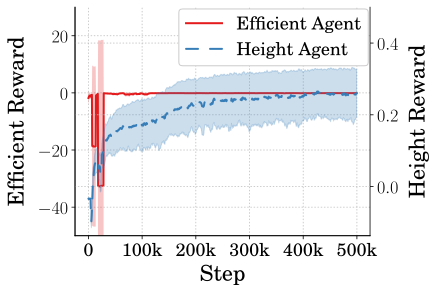
\includegraphics[width=\linewidth]{Figures/Ch2/RewVsTimeOne.png}
    \caption{Single Jumping Reward}
    \label{fig:avg_one_rew}
  \end{subfigure}%
  \hfill
  \begin{subfigure}{.49\textwidth}
    \centering
    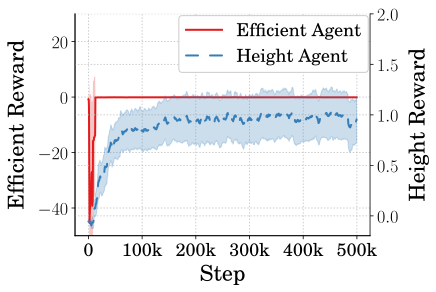
\includegraphics[width=\linewidth]{Figures/Ch2//RewVsTimeStutter.png}
     \caption{Stutter Jumping Reward}
     \label{fig:avg_stutter_rew}
  \end{subfigure}
   \caption{Reward vs Time Step During Training}
   \label{fig:avg_rew}
\end{figure}
% 

The average and standard deviation of the rewards during training for the efficient and high jumping strategies for both the single and stutter jumping commands are shown in Figure~\ref{fig:avg_rew}. They represent the controllers being trained to accomplish their respective goals. Looking at Figure~\ref{fig:avg_one_rew}, which shows the rewards for learning a single jumping command, it is clear that there are definite differences between the efficient and high-jumping reward types. Firstly, the high-jumping strategy does converge after 500k steps of training. The reward for the efficient-jumping controller, having been defined drastically different than the reward from the high-jumping controller, not surprisingly, looks drastically different than the high-jumping reward. The reward for the efficient agent is heavily punished for using power without gaining height, which is a frequent occurrence in the beginning of training. This forces the policy to learn that using less power will result in higher rewards within very few learning steps. In Figure~\ref{fig:avg_stutter_rew}, it is also apparent that the height controller converged to a solution. Additionally, the efficient controller can be seen to have learned in the same rapid form as the single jumping command type. 


\section{Average Performance of Network Controller}
\label{section:avg_performance}
% 
\subsection{Jumping commands}
\label{subsection:avg_input_performance}
% 
\begin{figure}[tb!]
  \centering
  \begin{subfigure}{.49\textwidth}
    \centering
    \includegraphics[width=\linewidth]{Figures/Ch2/avg_One_Input_.png}
    \caption{Single Jumping Input}
    \label{fig:avg_one_input}
  \end{subfigure}%
  \hfill
  \begin{subfigure}{.49\textwidth}
    \centering
    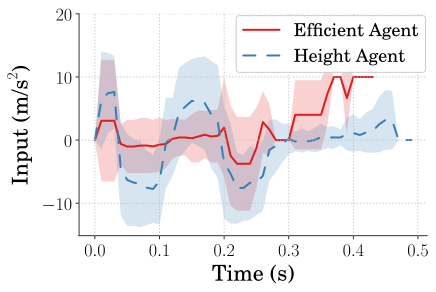
\includegraphics[width=\linewidth]{Figures/Ch2/avg_Stutter_Input_.png}
     \caption{Stutter Jumping Input}
     \label{fig:avg_stutter_input}
  \end{subfigure}
   \caption{Average and Standard Deviation Inputs to Monopode}
   \label{fig:avg_input}
\end{figure}
% 

The average and standard deviation of the final controller's commands for both the single and stutter jumping cases, and the results are shown in Figure~\ref{fig:avg_input}. At first glance, there are obvious differences regarding timing, magnitude, and direction. There are also slight differences in variance seen between the two controller types. 

Starting with Figure~\ref{fig:avg_one_input}, which displays the commands for the single jumping case, it is most obvious that the direction for the initial acceleration of the actuator mass differs between the efficient controllers and height controllers. In the case where the controller is learning to jump high, an initial acceleration of the actuator mass in the negative direction is learned, which contrasts the case where the controller is learning an efficient command. Further, the magnitude of the commands is drastically different which may be an indicator for conserving power. For the stutter jumping case, shown in Figure~\ref{fig:avg_stutter_input}, it is immediately apparent that the magnitudes of the commands differ greatly. They are, however, more similar in regards to their timing and directions than the single jumping command. 

In both the single and stutter jumping cases, it can be seen that there is upward acceleration command towards the end of the jump, which again, might be an indicator of a more efficient-jumping strategy. Furthermore, in the single jumping case, there exists more variance across different instances of the trained efficient controllers in comparison to the height controllers. This does not seem to be the case for the stutter jumping command type, though both cases do seem to generate controllers with high variance inputs across instances.
% 
\subsection{Jumping height performance}
\label{subsection:avg_height_performance}
% 
\begin{figure}[tb!]
  \centering
  \begin{subfigure}{.49\textwidth}
    \centering
    \includegraphics[width=\linewidth]{Figures/Ch2/avg_One_RodPos_.png}
    \caption{Single Jumping Height}
    \label{fig:avg_one_rodpos}
  \end{subfigure}%
  \hfill
  \begin{subfigure}{.49\textwidth}
    \centering
    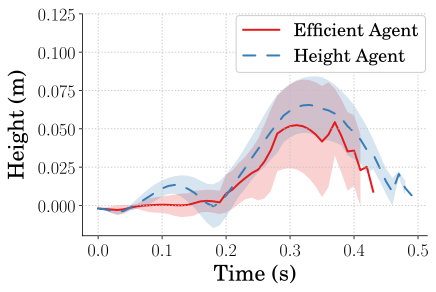
\includegraphics[width=\linewidth]{Figures/Ch2/avg_Stutter_RodPos_.png}
     \caption{Stutter Jumping Height}
     \label{fig:avg_stutter_rodpos}
  \end{subfigure}
   \caption{Average and Standard Deviation Heights of Monopode}
   \label{fig:avg_rodpos}
\end{figure}
% 

The average and standard deviation of the final jumping performance of the controllers are shown in Figure~\ref{fig:avg_rodpos}. In both the single and stutter jumping cases, there are differences in jumping ability when comparing the efficient and height controller types. It is apparent that when increasing the complexity of the command from a single jump to a stutter jump, the efficient controllers are better able to match the performance of the height controllers.

Shown in Figure~\ref{fig:avg_one_rodpos}, the height controllers for the single jumping case learned a command that outperformed the efficient controllers in terms of jump height. The resulting motion from the input discussed in the previous section can be seen in that the efficient controller learned to simply compress the spring, then jump the monopode. The height controllers, in contrast, disregarding power consumption, learned to decompress the spring from its nominal position, keeping it below the point of leaving the ground, then recompressing for a much higher jump. For the single jumping commands, the high-jumping strategy trained controllers that jumped the monopode 104.53\% higher than the efficient-jumping strategy, on average.
% Average Effective Height: 0.01520271583644785
% Average Height Height: 0.031095562970914627
% Percent Difference: 104.53952639412208

Figure~\ref{fig:avg_stutter_rodpos} compares the jumping performance of the efficient and height strategies for the stutter jumping command. They differ, but less drastically than the single jumping case. The similarity of the command shapes shown in Figure~\ref{fig:avg_stutter_input} results in jumping responses that also share a similar form. The large differences seen in the stutter jumping performance are similar to those seen in the inputs, in that they differ mostly regarding the magnitudes. For the stutter jumping command, the high-jumping strategy trained controllers that jumped the monopode 20.69\% higher than the efficient-jumping strategy, on average.
% Average Effective Height: 0.05431672664223123
% Average Height Height: 0.06555982552043371
% Percent Difference: 20.699146604060964

In both the single and stutter jumping cases, the upward acceleration from efficient controllers toward the end of the command can be seen in that the monopode regains height after the start of its final decent from maximum height. This can be explained in that the efficient control method, which punishes power consumption, discovered a way to maintain height throughout a jump where the utilization of additional power is less costly. It is less costly to influence the monopode's position while airborne because there is no resistance from the spring and damper. Additionally, regarding variance, the single jumping controllers seems to produce jumping shapes with similar levels of variance. Whereas in the stutter jumping case, though similar in high levels of input variance, the jumping height variance for the efficient controllers is noticeably higher than that of the height controller. This is likely because the reward for the efficient jumping strategy is fragile, and when learned, is difficult to optimize do to the extreme differences seen in the value received throughout training. A reward that deploys some normalization such that the value returned does not vary greatly would likely result in a better performing final policy.
% 
\subsection{Height reached vs. power used}
\label{subsection:avg_power_used}
% 
\begin{figure}[tb!]
    \centering
    \begin{subfigure}{.49\textwidth}
      \centering
      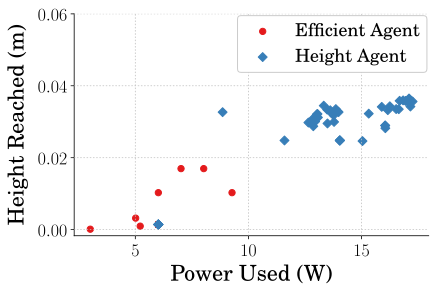
\includegraphics[width=\linewidth]{Figures/Ch2/One_HeightVsPower.png}
      \caption{Single Jumping Efficiency}
      \label{fig:single_heightvspower}
    \end{subfigure}%
    \hfill
    \begin{subfigure}{.49\textwidth}
      \centering
      \includegraphics[width=\linewidth]{Figures/Ch2/Stutter_HeightVsPower.png}
       \caption{Stutter Jumping Efficiency}
       \label{fig:stutter_heightvspower}
    \end{subfigure}
     \caption{Height Reached vs Power Consumed of Monopode}
     \label{fig:heightvspower}
\end{figure}
%

The height reached versus power consumed data for both the single jumping and stutter jumping cases, is shown in Figure~\ref{fig:heightvspower}. Although it looks as if there are less efficient instances, this is not the case. The efficient controller types simply learned more consistent control strategies, such that the data points lay on top of one another. This, again, is likely the result of innate fragility within the reward for the efficient controller. Regardless, in both the single and stutter jumping cases, the efficient controllers utilized less power and therefore suffered regarding jump height. This matches what was seen in the previous sections regarding commands and jumping shapes. In both jumping cases, the power conservation gain is greater than the jumping height cost. 

In the single jumping case, shown in Figure~\ref{fig:single_heightvspower}, there is an apparent separation between the two controller types where the height controllers learn control strategies that use more power and jump higher. On average, for the single jumping command type, the efficient-jumping strategy learned jumping commands that were 126.27\% more efficient at the cost of 104.53\% in average jump height.

As for the stutter jumping case, shown in Figure~\ref{fig:stutter_heightvspower}, the difference in performance is less obvious. This can be explained in that more complex jumping strategies give an RL algorithm more opportunity to learn a control policy that can better take advantage of system flexibility. The variance of the two controller types, being quite high, matches what is seen in the previous sections and results in more mixing of the data. On average, for the stutter jumping command type, the efficient strategy learned commands that were 101.45\% more efficient with the average maximum jumping height only being punished by 20.69\%.  
% One
% Average Efficient Power Used: 6.04808059689131
% Average Height Power Used: 13.685329381232417
% Percent Difference: 126.27557887152865
% Stutter
% Average Efficient Power Used: 7.756476293149168
% Average Height Power Used: 15.625778318248924
% Percent Difference: 101.45460035828692 

\section{Optimal Performance of the Proposed Controller}
\label{section:opt_performance}
% 
\subsection{Jumping commands}
\label{subsection:opt_input_performance}
% 
\begin{figure}[tb!]
    \centering
    \begin{subfigure}{.49\textwidth}
      \centering
      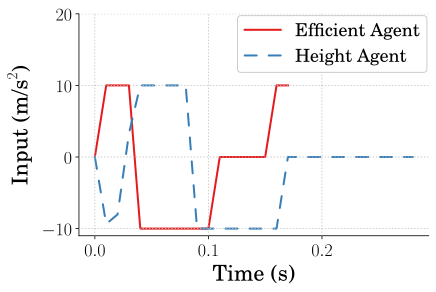
\includegraphics[width=\linewidth]{Figures/Ch2/best_One_Input_.png}
      \caption{Single Jumping Input}
      \label{fig:opt_one_input}
    \end{subfigure}%
    \hfill
    \begin{subfigure}{.49\textwidth}
      \centering
      \includegraphics[width=\linewidth]{Figures/Ch2/best_Stutter_Input_.png}
       \caption{Stutter Jumping Input}
       \label{fig:opt_stutter_input}
    \end{subfigure}
     \caption{Optimal Inputs to Monopode}
     \label{fig:opt_input}
\end{figure}
% 

Taking the best of the fifty different controllers trained for both the single and stutter jumping cases and comparing the efficient and height performance of the controllers can show what is possible with a properly defined RL problem. Figure~\ref{fig:opt_input} shows the differences in the commands generated when selecting the highest performing controller in terms of reward received. It can be seen that there are less differences between the efficient and height controllers in comparison to the average results from Section~\ref{section:avg_performance}. A major similarity is that magnitudes are similar across all cases such that the controllers utilize the maximum acceleration of the actuator. 

Looking at Figure~\ref{fig:opt_one_input}, which compares the efficient and height controllers for the single jumping input, the major differences are the timing and direction of the commands. This is similar to the average performance evaluation, from Section~\ref{subsection:avg_input_performance}, in that the efficient controller does not take advantage of the slight decompression of the spring before the monopode leaves the ground. Because of this, the efficient controller learns a different timing for a single jump. 

As for the stutter jumping case, shown in Figure~\ref{fig:opt_stutter_input}, the differences between the efficient and height controller are less drastic. The initial timing is largely the same as both controller types learn to utilize the decompression of the spring. The differences begin when decompressing the spring a second time and completing the first jump. The efficient controller learns a command similar in form to a bang-coast-bang command, where, in contrast, the height controller learns a command similar to that of a bang-bang shaped input. Bang-bang based commands have been shown to generate optimal jumping performance for high jumps for the monopode jumping system \cite{Vaughan2013}. Additionally bang-coast-bang shaped commands have been shown to be ones which could increase power efficiency \cite{doi:10.2514/2.4036}
% 
\subsection{Jumping height performance}
\label{subsection:opt_height_performance}
% 
\begin{figure}[tb!]
    \centering
    \begin{subfigure}{.49\textwidth}
      \centering
      \includegraphics[width=\linewidth]{Figures/Ch2/best_One_RodPos_.png}
      \caption{Single Jumping Height}
      \label{fig:opt_one_rodpos}
    \end{subfigure}%
    \hfill
    \begin{subfigure}{.49\textwidth}
      \centering
      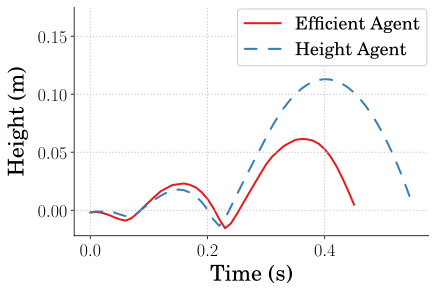
\includegraphics[width=\linewidth]{Figures/Ch2/best_Stutter_RodPos_.png}
       \caption{Stutter Jumping Height}
       \label{fig:opt_stutter_rodpos}
    \end{subfigure}
     \caption{Optimal Heights of Monopode}
     \label{fig:opt_rodpos}
\end{figure}
% 

Figure~\ref{fig:opt_rodpos} displays the jumping performance for both jump types as well as both controller types when utilizing the inputs shown in Section~\ref{subsection:opt_input_performance}. These curves show that the efficient controllers, in the best case scenario, do not generate commands that jump the monopode as high as the high jumping controllers.

Figure~\ref{fig:opt_one_rodpos}, which compares the efficient and height controllers for the single jump, shows that the efficient controller does not learn to utilize the allowable decompression in the spring. In Figure~\ref{fig:opt_stutter_rodpos}, it can be seen that when utilizing a command more similar in form to a bang-coast-bang command, like the efficient controller learned, the timing of the jump sequence is shifted and the resulting final height is less than the height controller where the command is more similar to a bang-bang shaped command. The efficient controller having learned to coast between commands shows it is a useful method for conserving power, but not a good strategy for optimizing jumping height. 
% One
% Max Efficient Height: 0.0169633024040252
% Max Height Height: 0.0364650959908489
% Percent Difference: 114.96460490025893
% Max Efficient Power Used: 8.023999999999997
% Max Height Power Used: 17.101847234287263
% Percent Difference: 113.13368936050934
% Stutter
% Max Efficient Height: 0.0607432013800848
% Max Height Height: 0.0915456169114579
% Percent Difference: 50.70923960466784
% Max Efficient Power Used: 17.93805315775764
% Max Height Power Used: 21.476888231927703
% Percent Difference: 19.72808890155189

\section{Conclusion}
Two different controller types were trained to generate two different jumping commands for the simplified monopode jumping system. The first type of controller was one that would command the monopode system to jump high where the reward was based on nothing other than system height. The second type of controller was one which controlled the monopode to jump high but at the cost of power consumed, such that high jumps that consumed high amount of power were less desirable than high jumps that consumed less power. It was shown that the rewards passed to RL algorithms that are training controllers can be manipulated so that the learned commands take advantage of the spring/damper that exists within the monopode jumping system. Furthermore, the timing of the commands, as well as the input magnitude and direction are all affected when defining a reward strategy that seeks to increase power efficiency. When considering the average performance of the different control strategies, for both the single and stutter jumping cases, the heights reached were less for the efficient strategies. However, they were significantly more efficient, particularly when scaling the complexity of the command from the single jump to the stutter jump. It should then be concluded that RL might serve as a useful method for defining control strategies for flexible-legged jumping systems, particularly when energy efficiency is of interest. Additionally, when considering more complex control strategies, which might be difficult to define efficiently, RL might serve as a useful method for effective efficient strategies.

%%%%%%%%%%%%%%%%
% Chapter 3
%%%%%%%%%%%%%%%%

%!TEX root = ULL_thesis_template.tex 
\chapter{Using Input Shaping to Validate RL Controllers}
\label{chapter3}
%
In utilizing RL to define a control strategy for a robotic system, the resulting commands sent to the system are often described as optimal, or at least approaching optimal. They are described as such due to the nature of RL problems in that the techniques used to learn a policy are optimization-theory based, so the policy being trained is one that is approaching an optimal solution in regards to the reward defined. Interpreting the commands claimed to be optimal, in the context of control theory, is an important part of utilizing RL for defining control strategies for robotic systems. In the case of a flexible jumping robot, where the command is to jump the system as high as possible or as efficiently as possible, the questions arises if the commands generated truly approach an optimal solution or not. To answer this question, the commands resulting from the trained agents can be analyzed leveraging conventional control theory. Methods such as input shaping have been shown to be effective for defining optimal control strategies for flexible jumping systems and can be used to evaluate the commands generated by the RL generated policies \cite{Vaughan2013}.

%%%%%%%%%%%%%%%%%%%%%%%%%%%%%%%%%%%%%%%%%%%%%%%%%%%%%%%%%%%%%%%%%%%%%%%%
%%%%%%%%%%%%%%%%%%%%%%%%%%%%%%%%%%%%%%%%%%%%%%%%%%%%%%%%%%%%%%%%%%%%%%%%
\section{Input Shaping Controller Input}
\label{sec:controller_input}
Bang-bang-based jumping commands like the one shown in Figure~\ref{fig:commandForm} are likely to result in a maximized jump height \cite{Vaughan2013}. For these command types, regarding the monopode jumping system, the actuator mass travels at maximum acceleration within its allowable range, pauses, then accelerates in the opposite direction. Commands designed to complete this motion are bang-bang in each direction, with a selectable delay between them. The resulting motion of the actuator along the rod is shown in Figure~\ref{fig:jumpingCommandPosition}. Starting from an initial position, $x_{a_0}$, the actuator moves through a motion of stroke length $\Delta_1$, pauses there for $\delta_t$, then moves a distance $\Delta_2$ during the second portion of the acceleration input.
%
\begin{figure}[tb!]
\centering
    \begin{subfigure}{0.45\columnwidth}
    \centering
    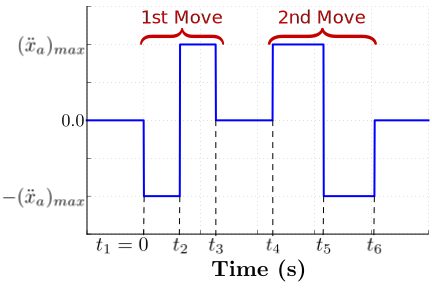
\includegraphics[width=\columnwidth]{Figures/Ch3/input_shaping/Command_form.pdf}
    \caption{Jumping Command \cite{Vaughan2013}}
    \label{fig:commandForm}
    \end{subfigure}
%
\hspace{0.05\columnwidth} % Optionally add some space between side-by-side figs
%
    \begin{subfigure}{0.45\columnwidth}
    \centering
    \includegraphics[width=\columnwidth]{Figures/Ch3/input_shaping/Jumping_command_position.pdf}
    \caption{Resulting Actuator Motion \cite{Vaughan2013}}
    \label{fig:jumpingCommandPosition}
    \end{subfigure}
\caption{Jumping Command Profiles} % Full figure caption
\label{fig:jumping_commands}	% Full figure label
\end{figure}
%

This bang-bang-based profile can be represented as a step command convolved with a series of impulses, as is shown in Figure \ref{fig:jumpConvolve} \cite{Sorensen2008CommandinducedVA}. Using this decomposition, input-shaping principles and tools can be used to both analyze and design the impulse sequence \cite{Singer:90, Singhose:94a}. For the bang-bang-based jumping command shown in Figure~\ref{fig:jumpConvolve}, the amplitudes of the resulting impulse sequence are fixed, $A_i = [-1, 2, -1, 1, -2, 1]$. The impulse times, $t_i$, can be varied and optimized leading to a maximized jump height of the monopode system \cite{Vaughan2013}. Commands of this form will often result in a stutter jump, like what was shown in Figure~\ref{fig:stutterJump} of Chapter~\ref{chapter2}, where the small initial jump allows the system to compress the spring to store energy to be used in the final jump. 
%
\begin{figure}[tb!]
  \centering
    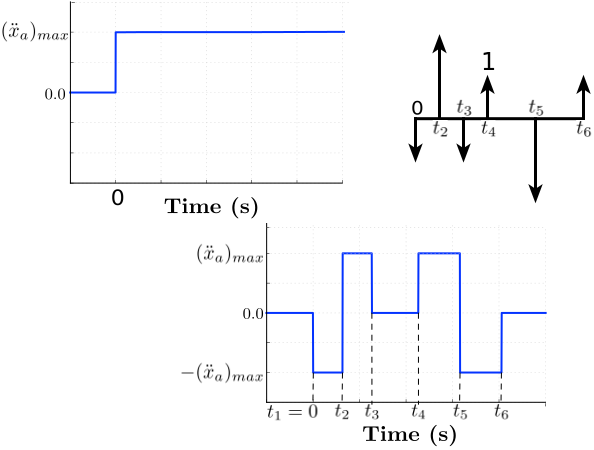
\includegraphics[width=0.75\textwidth]{Figures/Ch3/input_shaping/Jump_convolve.pdf}
    \caption{Decomposition of the Jump Command into a Step Convolved with an Impulse Sequence \cite{Vaughan2013}}
    \label{fig:jumpConvolve}
\end{figure}
%


%%%%%%%%%%%%%%%%%%%%%%%%%%%%%%%%%%%%%%%%%%%%%%%%%%%%%%%%%%%%%%%%%%%%%%%%
%%%%%%%%%%%%%%%%%%%%%%%%%%%%%%%%%%%%%%%%%%%%%%%%%%%%%%%%%%%%%%%%%%%%%%%%
\section{Review of Vector Diagrams}
\label{sec:vector_diagram_review}
%
One tool that seeks to simplify the design of impulse sequences for input shapers is the vector diagram \cite{Singhose:94a}. The vector diagram represents the vibration caused by an impulse as a vector, and the vibration induced by an impulse sequence as the sum of the representative vectors of the sequence. As such, the vector diagram can provide a visual means of both analysis and design of impulse sequences.

The process of plotting an impulse sequence on a vector diagram is shown in Figure~\ref{fig:vector_2imp}. 
%
\begin{figure}[tb!]
\begin{center}
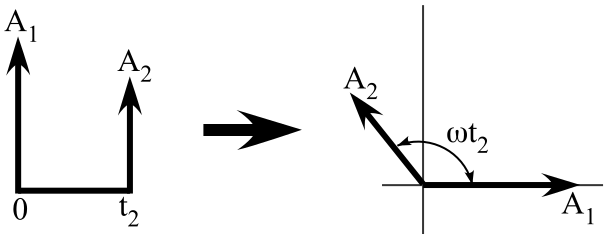
\includegraphics[width = 4.5in]{Figures/Ch3/input_shaping/vector_diagram_2imp}
\caption{Plotting Impulses on a Vector Diagram}
\label{fig:vector_2imp}
\end{center}
\end{figure}
%
Each impulse is plotted on the vector diagram in polar coordinates, where the magnitude of each vector is simply the impulse magnitude, and its angle is $\theta = \omega t_i$, where $\omega$ is the system natural frequency, and $t_i$ is the time location of the impulse.

To calculate the residual vibration caused by a sequence of impulses, the representative vectors are summed, as shown in Figure \ref{fig:vector_result}. 
%
\begin{figure}[tb!]
\begin{center}
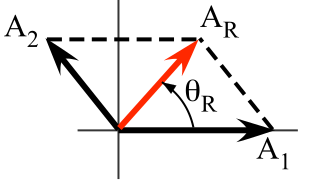
\includegraphics[width = 3in]{Figures/Ch3/input_shaping/vector_diagram_result}
\caption{Resultant Vibration Vector from Adding Impulses}
\label{fig:vector_result}
\end{center}
\end{figure}
%
The magnitude of the residual vibration caused by the sequence is proportional to the magnitude of the resultant vector, $A_R$.

The vector diagram can also be used as an input shaper design tool. For example, a third vector can be added to the sequence plotted in Figure \ref{fig:vector_result} to produce zero vibration. This third vector, $A_3$, could be placed opposite of $A_R$, as shown in Figure \ref{fig:vector_design_pos}. When $A_3$ is placed this way, the three vectors in the diagram sum to zero, indicating the impulse sequence will excite zero vibration at the design frequency and damping ratio.

To plot a negative impulse, the vector simply points toward the origin instead of away. Another option to design a zero vibration shaper from Figure \ref{fig:vector_result} is to place a negative impulse at $A_R$, as is shown in Figure \ref{fig:vector_design_neg}.
% 
\begin{figure}[tb!]
  \centering
  \begin{subfigure}[b]{0.45\textwidth}
    \centering
    \includegraphics[width=\textwidth]{Figures/Ch3/input_shaping/vector_diagram_design}
    \caption{Adding a Positive Impulse}
    \label{fig:vector_design_pos}
  \end{subfigure}
  \hfill
  \begin{subfigure}[b]{0.45\textwidth}
    \centering
    \includegraphics[width=\textwidth]{Figures/Ch3/input_shaping/vector_diagram_design_neg}
     \caption{Adding a Negative Impulse}
     \label{fig:vector_design_neg}
  \end{subfigure}
   \caption{Designing Input Shapers Using Vector Diagrams}
   \label{fig:vector_design}
\end{figure} 

In the context of this work, the vector diagram can be used to design an impulse sequence that \textit{maximizes} vibration. In other words, instead of arranging vectors to force $A_R$ toward zero, the vectors can be arranged to increase its magnitude. 


%%%%%%%%%%%%%%%%%%%%%%%%%%%%%%%%%%%%%%%%%%%%%%%%%%%%%%%%%%%%%%%%%%%%%%%%
%%%%%%%%%%%%%%%%%%%%%%%%%%%%%%%%%%%%%%%%%%%%%%%%%%%%%%%%%%%%%%%%%%%%%%%%
\section{Analysis of Learned Jumping Commands}
\label{sec:comparison_to_shaping}
%
In this section, the learned stutter-jumping commands for maximum jump height from Chapter~\ref{chapter2} will be analyzed using tools traditionally used for input shaping. This analysis will focus on the command shown previously in Figure \ref{fig:opt_stutter_input}. At first glance, the Height Agent command from this plot shares some similarities with the command introduced in Figure~\ref{fig:commandForm}. It is approximately two bang-bang commands.

A vector diagram of a single bang-bang command that maximizes vibration is shown in Figure~\ref{fig:bang_bang_vector}. The three impulses add constructively and indicate that a bang-bang command has the potential to excite three times the vibration of a single, unity-magnitude impulse (which is typically used as a proxy for the original reference command). The impulse sequence that is represented by the vector diagram is shown in Figure~\ref{fig:bang_bang_impulse}. The spacing of the impulses is such that the second, negative impulse should occur at $t_2 = \tau/2$ and the final impulse, $t_3$, at time $\tau$, where $\tau$ represents the system period ($\tau = 2\pi/\omega$).
% 
\begin{figure}[tb!]
  \centering
  \begin{subfigure}{0.5\textwidth}
    \centering
    \includegraphics[width=\textwidth]{Figures/Ch3/input_shaping/bang_bang_vector}
    \caption{Vector Diagram}
    \label{fig:bang_bang_vector}
  \end{subfigure}
  \hfill
  \begin{subfigure}{0.3\textwidth}
    \centering
    \includegraphics[width=\textwidth]{Figures/Ch3/input_shaping/bang_bang_impulses}
     \caption{Impulse Sequence}
     \label{fig:bang_bang_impulse}
  \end{subfigure}
   \caption{Maximum Vibration Bang-bang Impulse Sequence}
   \label{fig:bang_bang}
\end{figure} 

A vector diagram for a series of two bang-bang commands designed to maximize vibration is shown in Figure~\ref{fig:2x_bang_bang_vector}. This second bang-bang command in the sequence is just a repeat of the first, but beginning at time $\tau$, rather than at zero. The resulting impulse sequence is shown in Figure~\ref{fig:2x_bang_bang_impulse}
% 
\begin{figure}[tb!]
  \centering
  \begin{subfigure}{0.49\textwidth}
    \centering
    \includegraphics[width=\textwidth]{Figures/Ch3/input_shaping/2x_bang_bang_vector}
    \caption{Vector Diagram}
    \label{fig:2x_bang_bang_vector}
  \end{subfigure} 
  \hfill
  \begin{subfigure}{0.4\textwidth}
    \centering
    \includegraphics[width=\textwidth]{Figures/Ch3/input_shaping/2x_bang_bang_impulses}
     \caption{Impulse Sequence}
     \label{fig:2x_bang_bang_impulse}
  \end{subfigure}
   \caption{Maximum Vibration Dual Bang-bang Impulse Sequence}
   \label{fig:2x_bang_bang}
\end{figure} 
%
and can be written as:
\begin{equation}
\begin{bmatrix}A_i \\t_i\end{bmatrix} = \begin{bmatrix}1 & -2 & 1 & 1 & -2 & 1 \\[3pt] 0 & \frac{\tau}{2} & \tau & \tau & \frac{3\tau}{2} & 2\tau \end{bmatrix}
\label{eqn:2x_bang_bang_eq}
\end{equation}
%
where $A_i$ and $t_i$ represent the $i^{th}$ impulse amplitude and time, respectively. Given that the third and fourth impulses occur at the same time, the impulse sequence can further be simplified to:
%
\begin{equation}
\begin{bmatrix}A_i \\t_i\end{bmatrix} = \begin{bmatrix}1 & -2 & 2 & -2 & 1 \\[3pt] 0 & \frac{\tau}{2} & \tau & \frac{3\tau}{2} & 2\tau \end{bmatrix}.
\label{eqn:2x_bang_bang_eq_simple}
\end{equation}
%

The convolution of this impulse sequence with a step command in actuator acceleration, matching the process from Figure~\ref{fig:jumpConvolve}, is shown in Figure~\ref{fig:2x_bang_bang_conv}.
%
\begin{figure}[tb!]
\begin{center}
\includegraphics[width=0.85\textwidth]{Figures/Ch3/input_shaping/optimal_jump_convolve.pdf}  
\caption{Convolution of Maximum Vibration Bang-bang Impulse Sequence}
\label{fig:2x_bang_bang_conv}
\end{center}
\vspace{-0.2in}
\end{figure}
%
The resulting jumping response is shown in Figure~\ref{fig:optimum_jump} in comparison to the jumping response of the best high jumping agent from Chapter~\ref{chapter2}.
%
\begin{figure}[tb!]
  \centering
      \begin{subfigure}{0.49\columnwidth}
      \centering
      \includegraphics[width=\columnwidth]{Figures/Ch3/input_shaping/learned_comparison_to_optimal_command.pdf}  
      \caption{Jumping Commands}
      \label{fig:optimum_jump_command}
      \end{subfigure}
      \hfill
      \begin{subfigure}{0.49\columnwidth}
      \centering
      \includegraphics[width=\columnwidth]{Figures/Ch3/input_shaping/learned_comparison_to_optimal_response.pdf}  
      \caption{Jumping Responses}
      \label{fig:optimum_jump_response}
      \end{subfigure}
  \caption{Input and Jumping Response for Maximum Vibration Bang-bang Impulse Sequence} % Full figure caption
  \label{fig:optimum_jump}	% Full figure label
  \end{figure}
  %
This case represents the upper bound of the jump height possible for a linearized version of the monopode system, given the actuator limits imposed. While the form of the command in Figure~\ref{fig:2x_bang_bang_conv} is similar to that learned by the RL algorithm, shown in Figure~\ref{fig:opt_stutter_input}, the timing of the transitions between negative and positive acceleration are slightly different, particularly toward the end of the command. The input command, not having knowledge of the system through learning, fails to stutter jump the system. This happens as a result of the command timing not aligning with the position of the system. Looking at the timing in Figures~\ref{fig:optimum_jump_command} and~\ref{fig:optimum_jump_response}, it can be seen that the second positive acceleration ends too quickly without fully compressing the spring. With the spring not being fully compressed the system is still accelerating in the negative direction, so when the final negative acceleration is sent, the system simply decelerates and oscillates until the time limit is reached.

If the command learned by the agent in Figure~\ref{fig:opt_stutter_input} is analyzed directly, an impulse sequence representing its bang-bang profiles can be found to be:
%
\begin{equation}
\begin{bmatrix}A_i \\t_i\end{bmatrix} \approx \begin{bmatrix}1 & -2 & 2 & -2 & 1 \\[3pt] 0 & \frac{\tau}{2} & \tau & 2\tau & 3\tau \end{bmatrix}
\label{eqn:rl_match_impulses}
\end{equation}
%
A vector diagram of this sequence of impulses is shown in Figure~\ref{fig:rl_match_vector}. From the vector diagram, the resultant vector does not reach the amplitude of the theoretical upper-bound case, but does result in vibration that is 400\% of that which a single, unity magnitude impulse would create.
%
\begin{figure}[tb!]
\begin{center}
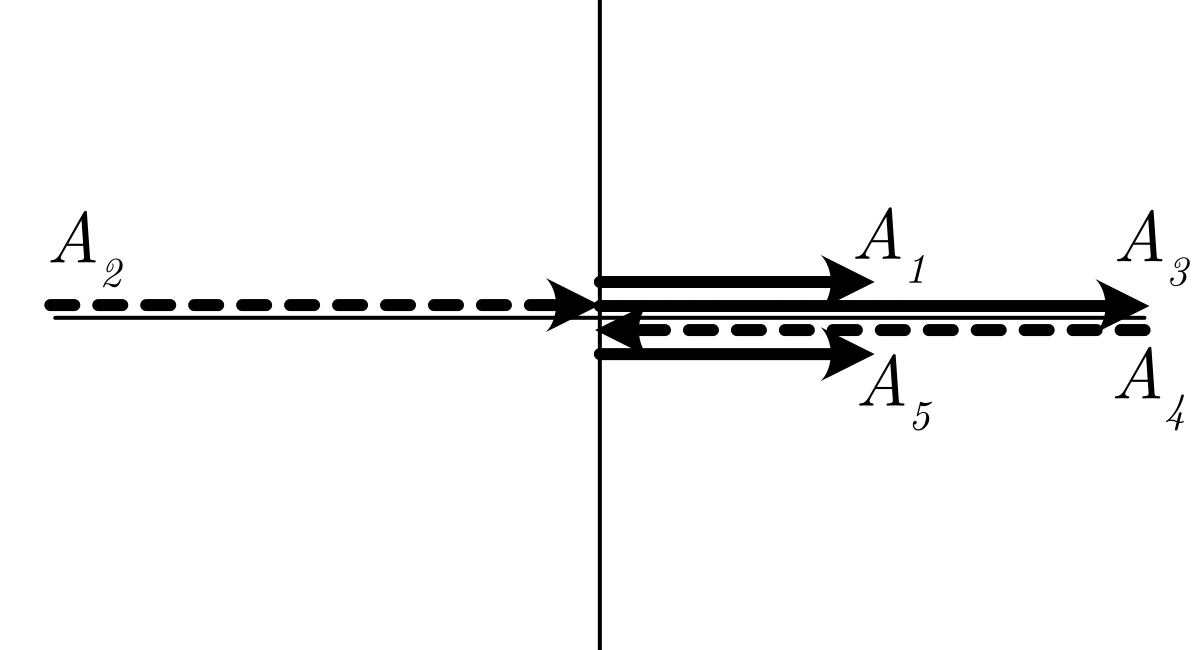
\includegraphics[width = 4in]{Figures/Ch3/input_shaping/rl_bang_bang_vector.pdf}
\caption{Vector Diagram for Learned Jumping Command}
\label{fig:rl_match_vector}
\end{center}
\vspace{-0.2in}
\end{figure}
%

The learned command and the one resulting from the convolution of this impulse sequence are shown in Figure~\ref{fig:learned_shaped_command_comparison}. The timing and amplitude of the command generated using the impulse sequence are a good match for the learned policy. This is further confirmed by comparing the jumping responses for the two commands, which are shown in Figure~\ref{fig:learned_shaped_response_comparison}.
%
\begin{figure}[tb!]
\centering
    \begin{subfigure}{0.49\columnwidth}
    \centering
    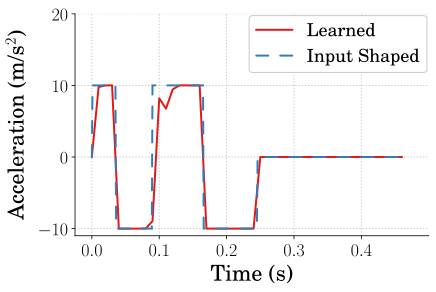
\includegraphics[width=\columnwidth]{Figures/Ch3/input_shaping/learned_shaped_command_comparison.pdf}  
    \caption{Jumping Commands}
    \label{fig:learned_shaped_command_comparison}
    \end{subfigure}
    \hfill
    \begin{subfigure}{0.49\columnwidth}
    \centering
    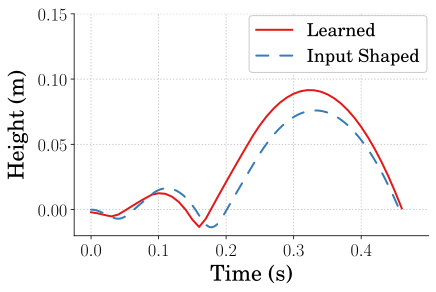
\includegraphics[width=\columnwidth]{Figures/Ch3/input_shaping/learned_shaped_response_comparison.pdf}  
    \caption{Jumping Responses}
    \label{fig:learned_shaped_response_comparison}
    \end{subfigure}
\caption{Comparison of Learned Controller and Input Shaping Approximation} % Full figure caption
\label{fig:rl_shaping_comparison}	% Full figure label
\end{figure}
%

In Figure~\ref{fig:learned_shaped_response_comparison}, the learned controller achieves a slightly greater jump height than the input-shaped approximation of it, but the general trends between the two match. The disparity in height is likely do to the input-shaped command being defined for a linear approximation of the monopode jumping system, whereas the RL-policy was trained on the nonlinear system. Both commands were evaluated on the nonlinear system. Regardless of the disparities, the results confirm that the methods presented in this chapter are a feasible option for analyzing control strategies learned using RL techniques.

%%%%%%%%%%%%%%%%%%%%%%%%%%%%%%%%%%%%%%%%%%%%%%%%%%%%%%%%%%%%%%%%%%%%%%%%
%%%%%%%%%%%%%%%%%%%%%%%%%%%%%%%%%%%%%%%%%%%%%%%%%%%%%%%%%%%%%%%%%%%%%%%%
\section{Conclusion}
%
An approach to design jumping commands using input shaping was reviewed. Then, the best learned stutter jumping command from Chapter~\ref{chapter2} was analyzed using methods approximating the command with an input-shaped step command. This analysis showed that the RL-learned command does not directly match the theoretical maximum for a linearized model of the monopode system. However, both the commands and responses for the shaped approximation and the RL agent matched closely, suggesting that input shaping is a feasible option for the analysis of learned policies.

%%%%%%%%%%%%%%%%
% Chapter 4
%%%%%%%%%%%%%%%%

%!TEX root = ULL_thesis_template.tex 
\chapter{Mechanical Design of a the Monopode Jumping System}
\label{chapter4}

Often it is the goal of a controls engineer to design a controller to accommodate and manipulate systems according to the system description provided. However, research has been conducted showing the value of studying the manipulation of mechanical design parameters in order to achieve a desired system behavior \cite{Li2001}. In this chapter, reinforcement learning is shown to be useful as a tool to learn mechanical designs given a predefined system controller for the monopode jumping system. RL has been shown to be an effective strategy for finding optimal concurrent designs for many different types of systems \cite{Schaff2019e, Luck2019, Ha2019j}. It has even shown its ability to define designs that are successfully deployed on physical hardware \cite{Chen2020}. It is comparable to work where evolutionary algorithms are deployed to optimize physical parameters of systems for improved energy efficiency \cite{Wang2019, Hu2020}. Here, RL is used to define an optimal design for the monopode jumping system described in Chapter~\ref{chapter2}.

\section{Learning a Mechanical Design}
Section~\ref{sec:rl} describes the common deployment methodology of an RL problem where defining a control policy for a robotic system is often the primary goal. In this chapter, rather than finding a control policy for a defined robotic system, RL is deployed to find a mechanical design for a defined control input. To do this, the general methods in setting up the problem have to change. Figure~\ref{fig:TD3_mech_design} shows the general flow of information for the algorithm.

% 
\begin{figure}[tb!]
        \centering
        \includegraphics[width=0.95\textwidth]{figures/Ch4/TD3_Mech_Params.drawio.png}  
        \caption{Learning a Mechanical Design}
        \label{fig:TD3_mech_design}
\end{figure}
% 

The RL problem is similar to the common use case in that the algorithm utilizes the same information types to optimize a design, such as the state of the environment and the reward. The interaction of the algorithm with the environment is drastically different, however. The action space, instead of being a command type input, is a range of design choices for a set of parameters within a simulation of a system. Applying these actions within the environment, rather than changing the state of a robotic system from state $s$ to $s'$, instead simulates a system within the environment from time $t=0$ to time $T$ using a predefined control input. Because of this, the state saved as a transition is a matrix of states rather than a single vector state. The reward does not differ greatly in that it is based on the state of the system. The difference is that the information stored in a single state transition is much greater so the reward can be defined to utilize all the information.

For the work presented in this chapter, the predefined control input used to simulate the monopode system within the environment at each step was an optimized controller generated using the input shaping techniques discussed in Section~\ref{sec:controller_input} as is shown in Figure~\ref{fig:TD3_mech_design}. Having been shown to be a useful technique for generating optimal control strategies, it was of interest to evaluate if an optimal mechanical design could be found to accompany the input.

\section{Environment Definition}
To allow the agent to find a mechanical design, a reinforcement learning environment conforming to the OpenAI Gym standard \cite{Brockman2016c} was created. The monopode model described in Chapter~\ref{chapter2} was used as the simulation, and the fixed controller input was based on the work described in Section~\ref{sec:controller_input}. The mechanical parameters the agent was tasked with optimizing were the spring constant and the damping ratio of the monopode system. At each episode during training, the policy of the algorithm selected a set of design parameters from a distribution of predefined parameter ranges and saved the timeseries simulation information in the replay buffer. The actions applied, $\mathcal{A}$, within the environment were the designs selected and were defined as follows:
% 
\begin{equation}
    \label{eq:mech_action}
    \begin{aligned}
    \mathcal{A} = \{ \{ a_{\alpha} \in \mathbb{R}: [0.1 \alpha_{nom}, 1.9 \alpha_{nom}] \}, \, \{ a_{\zeta} \in \mathbb{R}: [0.1 \zeta_{nom}, 1.9 \zeta_{nom}] \} \}
    \end{aligned}
\end{equation}
% 
where $\alpha_{nom}$ and $\zeta_{nom}$ are the nominal spring constant and damping ratio of the monopode, respectively; $x_t$ and $\dot{x}_t$ are the rod height and velocity steps of the monopode, and $x_{a_t}$ and $\dot{x}_{a_t}$ are the actuator position and velocity steps of the monopode, all captured during simulation. The action space was set to $\pm$90\% of the nominal values as that percentage allowed for a large variance in performance across the range of designs. The observations saved, were the timeseries information, and were defined as:
% 
\begin{equation}
    \label{eq:mech_transitions}
    \mathcal{S}= \{ \textup{\textbf{X}}, \dot{\textup{\textbf{X}}}, \textup{\textbf{X}}_a, \dot{\textup{\textbf{X}}}_a \}
\end{equation}
% 
where $\textup{\textbf{X}}$, $\dot{\textup{\textbf{X}}}$, $\textup{\textbf{X}}_a$ and $\dot{\textup{\textbf{X}}}_a$ are timeseries data for the position and velocity of the rod, and the position and velocity of the actuator, respectively.


\section{Rewards for Learning Designs}
The RL algorithm was utilized to find designs for two different reward cases. Time series data was captured during the simulation phase of training and was used to evaluate the designs performance through these rewards. The first reward case used was:
%
\begin{equation}
        R_1 = \left \{ \textup{\textbf{X}} \right \}_{\textup{max}}
\end{equation}
% 
where $x_t$ was the rod height of the monopode at each step during simulation. The goal of the first reward was to find a design that would cause the monopode to jump as high as possible. 

The reward for the second case was:
%
\begin{equation}
        R_2 = \frac{1}{\frac{\left | \mathbb{R}_1 - x_s \right |}{x_s} + 1}
\end{equation}
%
where $x_s$ was the desired jump height, which was set to 0.1~m. The second case was utilized to test ability of RL to find a design that minimized the error between the maximum height reached and the desired maximum height to reach.

\section{Design Space Variations}
% 
\begin{figure}[tb!]
        \centering
        \begin{subfigure}{0.75\textwidth}
        \centering
        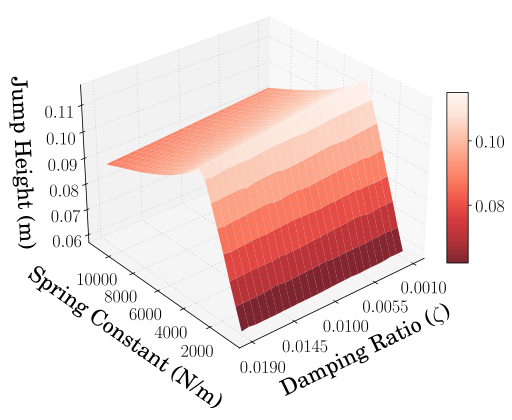
\includegraphics[width=\linewidth]{figures/Ch4/design_space_narr/Design_3D_Plot_0.01_.pdf}
        \caption{Jumping Performance of Narrow Design Space}
        \label{fig:spring_zeta_narr}
        \end{subfigure} \\
        \begin{subfigure}{0.75\textwidth}
        \centering
        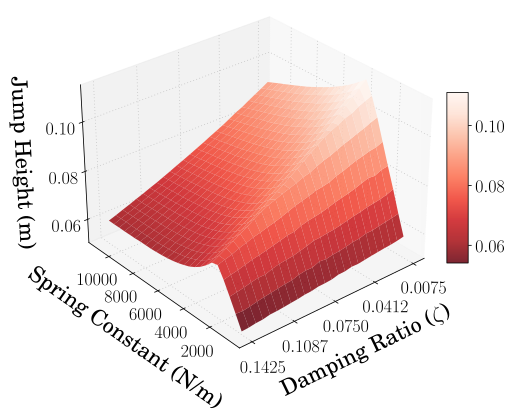
\includegraphics[width=\linewidth]{figures/Ch4/design_space_wide/Design_3D_Plot_0.075_.pdf}
        \caption{Jumping Performance of Wide Design Space}
        \label{fig:spring_zeta_wide}
        \end{subfigure} 
         \caption{Reference Jumping Performance of the Monopode}
         \label{fig:spring_vs_zeta}
\end{figure}

Figure~\ref{fig:spring_vs_zeta} represents the heights the monopode could reach for two different design spaces. The design space provided for the first case, shown in Figure~\ref{fig:spring_zeta_narr}, represents a space where the nominal damping ratio, $\zeta_{nom}$, is $0.01$, such that $\pm0.9 \, \zeta_{nom}$ creates a more narrow design space. This design space also has more values closer to the optimal value therefore making it more difficult to optimize quickly. The design space provided for the second case, shown in Figure~\ref{fig:spring_zeta_wide}, represents a space where the nominal damping ratio, $\zeta_{nom}$, is $0.075$, such that $\pm0.9 \, \zeta$ creates a wider design space. Additionally, there is a more obvious maximum within the design space, making it easer to ascend towards an optimal design. In both cases there are many values that would satisfy the specified height jumping strategy.

\section{Deploying TD3}
% 
\begin{table}[tb!]
\caption{TD3 Training Hyperparameters}
\begin{center}
\vspace{-12pt}
\begin{tabular}{c c}
\textbf{Hyperameter}            & \textbf{Value}                  \\
\hline
\hline
Learning Rate, $\alpha$         & 0.001                           \\
Learning Starts                 & 100 Steps                       \\
Batch Size                      & 100 Transitions                 \\
Tau, $\tau$                     & 0.005                           \\
Gamma, $\gamma$                 & 0.99                            \\
Training Frequency              & 1:Episode                       \\
Gradient Steps                  & $\propto$ Training Frequency    \\
Action Noise,  $\epsilon$       & None                            \\
Policy Delay                    & 1 : 2 Q-Function Updates        \\
Target Policy Noise, $\epsilon$ & 0.2                             \\
Target Policy Clip, $c$         & 0.5                             \\
Seed                            & 100 Random Seeds                \\
\hline
\hline
\end{tabular}
\label{tab:mech_hyperparams}
\end{center}
\end{table}
%
% \begin{figure}[tb!]
%         \centering
%         \includegraphics[width=0.75\textwidth]{figures/Ch4/design_space_wide/RewVsTime_2021-10-12_144814.pdf}  
%         \caption{Reward Received During Training}
%         \label{fig:rew_vs_step_narr}
% \end{figure}
% %
% \begin{figure}[tb!]
%         \centering
%         \includegraphics[width=0.75\textwidth]{figures//Ch4/design_space_narr/RewVsTime_2021-10-12_145004.pdf}  
%         \caption{Reward Received During Training}
%         \label{fig:rew_v_step_wide}
% \end{figure}   

The training hyperparameters were selected based on the author of TD3 recommendations and \textbf{StableBaselines3} \cite{stable-baselines3} experimental findings and are displayed in Table~\ref{tab:mech_hyperparams}. All of the hyperparameters, with the exception of the rollout (Learning Starts) and the replay buffer, were set according to \textbf{StableBaselines3} standards. The rollout setting was defined such that the agent could search the design space at random, filling the replay buffer with enough experience to prevent the agent from converging to a design space that was not optimal. The replay buffer was sized proportional to the number of training steps due to system memory constraints. 

%
\begin{figure}[tb!]
        \centering
        \begin{subfigure}{.49\textwidth}
          \centering
          \includegraphics[width=\linewidth]{figures/Ch4/design_space_narr/RewVsTime.png}
          \caption{Reward vs. Episode: Narrow Design Space}
          \label{fig:rew_vs_step_narr}
        \end{subfigure}%
        \hfill
        \begin{subfigure}{.49\textwidth}
          \centering
          \includegraphics[width=\linewidth]{figures/Ch4/design_space_wide/RewVsTime.png}
           \caption{Reward vs. Episode: Wide Design Space}
           \label{fig:rew_v_step_wide}
        \end{subfigure}
         \caption{Reward vs. Episode for Learning Mechanical Design}
         \label{fig:rew_vs_step}
\end{figure}
%    

The average rewards for both the narrow and the wide design space agents are shown in Figure~\ref{fig:rew_vs_step}. They represent the agents learning a converging solution to the problem of finding optimal design parameters. Looking at Figure~\ref{fig:rew_vs_step_narr}, it is apparent that given a more narrow design space, both the high and the specified jumping agents were still able to learn a converging solution. There also exists more variance for the specified-height agent type compared to the agents assigned with maximizing jump height. Looking at Figure~\ref{fig:rew_v_step_wide}, it is apparent that the agents given a wider design space where both able to learn a converging design solution. Though, given more designs to choose from, it appears the specified height agents are taking longer to converge. Additionally, once converged, because there are less values that allow the controller/design architecture to accomplish the tasks, there is less variance seen in the learned designs.

\section{Jumping Performance}
\subsection{Narrow design space}

Figure~\ref{fig:height_v_step_narr} shows the height achieved by the learned designs for the agents given the narrow range of possible damping ratio values. For the agents learning designs to maximize jump height, Figure~\ref{fig:height_v_step_narr} can be compared with Figure~\ref{fig:spring_zeta_narr} showing that the agent learned a design nearing one which would achieve maximum performance. Additionally, looking at the agents learning designs to jump to the specified 0.1~m, the learned designs accomplish this with slightly more variance than that of the maximum height case.
% 
\begin{figure}[tb!]
        \centering
        \includegraphics[width=0.75\textwidth]{figures/Ch4/design_space_narr/HeightVsTime.png}  
        \caption{Height Reached During Training Given Narrow Design Space}
        \label{fig:height_v_step_narr}
\end{figure}
% 

%  
\begin{figure}[tb!]
        \centering
        \begin{subfigure}{.49\textwidth}
                \centering
                \includegraphics[width=\textwidth]{figures/Ch4/design_space_narr/SpringVsTime.png}  
                \caption{Spring Constant Selected During Training}
                \label{fig:spring_v_step_narr}
        \end{subfigure}%
        \hfill
        \begin{subfigure}{.49\textwidth}
                \centering
                \includegraphics[width=\textwidth]{figures/Ch4/design_space_narr/ZetaVsTime.png}  
                \caption{Damping Ratio Selected During Training}
                \label{fig:zeta_v_step_narr}
        \end{subfigure}
         \caption{Designs Learned for the Narrow Design Space}
         \label{fig:des_vs_step_narr}
\end{figure}
% 

The average and standard deviation of the spring constant and damping ratio design parameters the agents selected during training are shown in Figure~\ref{fig:des_vs_step_narr}. These plots represent the learning curves for the agents learning design parameters to maximize jump height and the agents learning design parameters to jump to 0.1~m. There is a high variance in both the spring constant and the damping ratio found for the agents that learned designs to jump to a specified height. The agents which were learning designs that maximized height found designs with very little variance in terms of spring constant. In regards to the damping ratio, the agents learning designs for a specified height found designs with significantly more variances compared to the agents learning designs for the maximized height.

\subsection{Wide design space}
%
\begin{figure}[tb!]
        \centering
        \includegraphics[width=0.75\textwidth]{figures//Ch4/design_space_wide/HeightVsTime.png}  
        \caption{Height Reached During Training Given Wide Design Space}
        \label{fig:height_v_step_wide}
\end{figure}
%

Figure~\ref{fig:height_v_step_wide} shows the height achieved by the learned designs for the agents given a wide range of damping ratios. For the agents learning designs to maximize jump height, Figure~\ref{fig:height_v_step_wide} can be compared with Figure~\ref{fig:spring_zeta_wide} showing that the agents learned a design nearing one which would achieve maximum performance. Additionally, looking at the agents learning designs to jump to the specified 0.1~m, the learned designs accomplish this, again, only with slightly more variance than what is seen in the maximum height agents. 
%  
\begin{figure}[tb!]
        \centering
        \begin{subfigure}{.49\textwidth}
                \centering
        \includegraphics[width=\textwidth]{figures//Ch4/design_space_wide/SpringVsTime.png}  
        \caption{Spring Constant Selected During Training}
        \label{fig:spring_v_step_wide}
        \end{subfigure}%
        \hfill
        \begin{subfigure}{.49\textwidth}
                \centering
        \includegraphics[width=\textwidth]{figures//Ch4/design_space_wide/ZetaVsTime.png}  
        \caption{Damping Ratio Selected During Training}
        \label{fig:zeta_vs_step_wide}
        \end{subfigure}
         \caption{Designs Learned for the Wide Design Space}
         \label{fig:des_vs_step_wide}
\end{figure}
%

The average and standard deviation of the spring constant and damping ratio design parameters the agents selected during training are shown in Figure~\ref{fig:des_vs_step_wide}. For the agents that learned designs to jump to a specified height, it can be seen that there is significantly higher variance regarding the spring constant throughout training compared to the agent learning a design to maximize height. However, after 1000 iterations, the majority of agents converge to a specific design, lowering the variance. The same can be seen in the damping ratio; however, the variance is mitigated significantly earlier in training. The agents which were learning designs that maximized height found them with very little variance in terms of spring constant and damping ratio. 
% 
\subsection{Average design performance}
% 
\begin{table*}[tb!]
\caption{Learned Design Parameters}
\vspace{-4mm}
\label{tab:learned_design_params}
\begin{center}
\begin{tabular}{c c c c c}
\multicolumn{2}{c}{\textbf{Training Case}}                                                                 & \textbf{Design Parameter} & \textbf{Mean}     & \textbf{STD}      \\
\hline
\hline
\multirow{4}{*}{\centering Narrow Design Space}         & \multirow{2}{*}{\centering Max Height}             & Spring Constant           & 3.62e03           & 3.82e01           \\
                                                        &                                                    & Damping Ratio             & 3.37e-04          & 2.11e-03          \\
                                                        & \multirow{2}{*}{\centering Specified Height}       & Spring Constant           & 7.74e03           & 1.24e03           \\
                                                        &                                                    & Damping Ratio             & 4.55e-03          & 6.49e-03          \\
\multirow{4}{*}{\centering Broad Design Space}          & \multirow{2}{*}{\centering Max Height}             & Spring Constant           & 3.55e03           & 4.86e01           \\
                                                        &                                                    & Damping Ratio             & 7.53e-03          & 8.86e-06          \\
                                                        & \multirow{2}{*}{\centering Specified Height}       & Spring Constant           & 7.07e03           & 2.16e02           \\
                                                        &                                                    & Damping Ratio             & 7.54e-03          & 3.27e-05          \\
\hline
\hline
\end{tabular}
\end{center}
\end{table*}

The final mean and standard deviation of the design parameters for the two different cases are presented in Table~\ref{tab:learned_design_params}. Figure~\ref{fig:height_vs_time} shows the jumping performance of the mean learned designs for both cases tested. The agents tasked with finding designs to jump to the specified 0.1~m, did so with minimal error. The difference seen in maximum height reached between the two cases represents the difference in the nominal damping ratio within the design spaces. The peak heights from Figure~\ref{fig:height_vs_time} for the maximum height designs can be compared to Figures~\ref{fig:spring_zeta_narr} and~\ref{fig:spring_zeta_wide} to show that the agents learned designs nearing those achieving maximum performance. 
%
\begin{figure}[tb!]
        \centering
        \includegraphics[width=0.75\textwidth]{figures/Ch4/timeseries/TimeseriesHeight.png}  
        \caption{Height vs Time of Average Optimal Designs}
        \label{fig:height_vs_time}
\end{figure}
% 
\begin{figure}[tb!]
        \centering
        \begin{subfigure}{0.75\textwidth}
        \centering
        \includegraphics[width=\linewidth]{figures/Ch4/design_space_narr/3D_Plot_0.01_.pdf}
        \caption{Average Design Performance Within Narrow Design Space}
        \label{fig:des_performance_wide}
        \end{subfigure} \\
        \begin{subfigure}{0.75\textwidth}
        \centering
        \includegraphics[width=\linewidth]{figures/Ch4/design_space_wide/3D_Plot_0.075_.pdf}
        \caption{Average Design Performance Within Wide Design Space}
        \label{fig:des_performance_narrow}
        \end{subfigure} 
         \caption{Reference Jumping Performance of the Monopode}
         \label{fig:des_performance}
\end{figure}

Additionally, Figure~\ref{fig:des_performance} shows the average designs, and their performance, against the design space performance data. It is apparent that in the case of the narrow design space, where the optimal design for maximizing height is more prominent, the design found is one that is approaching optimal performance. In the case of the wide design space, where the design that optimizes height is less prominent, it is apparent that the design found by the agent is only nearing the optimal design. In both design space cases, the design found to force the monopode to jump to the specified height was found within the higher values of the spring constant range, even though values did exist in the lower range that would satisfy the jumping condition.

\section{Conclusion}
The monopode model was used in conjunction with a predetermined control input to determine if a reinforcement learning algorithm (TD3) could be used to find optimal performing design parameters regarding jumping performance. This work was done in part to determine if reinforcement learning could be used as the mechanical design learner for an intelligent concurrent design algorithm. It was shown that when providing an agent with a design space that was smaller in size with a more prominent optimal value, the agents performed well in finding design parameters which met the performance constraints. The designs found were lower in variance as well, even in the in the case where the algorithm was tasked with finding a design for a specific performance within the range of possible performances. It was additionally shown that when provided with a larger design space, that additionally had many values closer to the optimal value, the agents still excelled at finding design parameters that performed close to optimal. The parameters found were higher in variance however, as expected, particularly in the case where a design was to be found to generate a specific performance. This was due to the number of design options that would satisfy the performance requirements. It should be concluded ultimately that utilizing an RL algorithm, such as TD3, for the mechanical design aspect of a concurrent design method, is a viable solution.

%%%%%%%%%%%%%%%%
% Chapter 5
%%%%%%%%%%%%%%%%

%!TEX root = ULL_thesis_template.tex 
\chapter{Concurrent Design of the Monopode System}
\label{chapter5}

The workflow for creating a mechanical system and associated control strategy is often sequential. Typically, the mechanical and electrical hardware are developed, creating a set of confinements for the controller to be designed from. However, the mechanical/electrical system description is not always a simple one, and generating a controller for it might be unnecessarily challenging. Allowing the mechanical/electrical parameters of the system, and therefore the system's description, to be changeable could be valuable. This would allow for optimization of the complete system rather than optimizing the mechanical/electrical elements and control in isolation. Designing the system and control input in unison has been researched and is often referred to as concurrent design. This strategy has been used to develop better performing mechatronics systems \cite{Li2001}. More recent work has used advanced methods such as evolutionary strategies to select robot design parameters \cite{Wang2019}. In addition to evolutionary strategies, reinforcement learning has been shown to be a viable solution for concurrent design of 2D simulated locomotive systems \cite{Ha2019j}. This is further shown to be a viable method by demonstrating more complex morphology modifications in 3D reaching and locomotive tasks \cite{Schaff2019e}. However, these techniques have not yet been applied to flexible systems for locomotive tasks. In this chapter, a concurrent design architecture is proposed to find an optimal design and controller for the monopode jumping system defined in Chapter~\ref{chapter2}. 
%-----------------------------------------------------
\section{Concurrent Design Architecture}
\label{sec:concurrent_des_arch}
% 
\begin{figure}[tb!]
  \centering
  \includegraphics[width=\textwidth]{figures/Ch5/conc_des_diagram.drawio.png}  
  \caption{Concurrent Design Architecture}
  \label{fig:conc_des_diagram}
\end{figure}
% 

To define a concurrent design process utilizing RL, the proposed algorithm uses two instances of the TD3 algorithm, creating an inner and an outer loop. The first instance, which is responsible for learning the control policy, will be instantiated in a similar fashion to the what was seen in Chapter~\ref{chapter2}. It is the outer loop of the concurrent design process. The second instance, which is responsible for learning the mechanical design, is instantiated in the inner loop and in a similar fashion to what was seen in Chapter~\ref{chapter4}. A key aspect of the inner loop instantiation is that rather than using a pre-defined control input, like what was shown in Chapter~\ref{chapter4}, the simulation used the input that was being trained by the outer loop instantiation. Figure~\ref{fig:conc_des_diagram} shows the general flow of information for the concurrent design algorithm. The inner loop, replicating the work from Chapter~\ref{chapter4}, is within the ``Update Design'' block. The description of the inner loop was shown in Figure~\ref{fig:TD3_mech_design}, only the defined input that was used in Chapter~\ref{chapter4} was replaced in this diagram by the current policy, $\pi$. A detailed algorithm, describing the process presented in Figure~\ref{fig:conc_des_diagram}, is presented in Appendix~\ref{app:concurrent_des_algo}. 

%-----------------------------------------------------
\section{Mechanical Design Update}
\subsection{Discrete vs. continuous}
As is further discussed in Appendix~\ref{app:concurrent_des_algo}, there are two different methods for implementing the inner loop of the concurrent design algorithm. The first is called the \textit{discrete} method, where at each environment design update, the model learning the design is instantiated fresh and learns a design from scratch. The second method is called \textit{continuous}, where at each environment update the model learning the design is saved and reloaded so that the model that is learning a design is the same over the course of the controller model training. 

\subsection{Averaging design policies}
In Chapter~\ref{chapter4}, average designs found from 50 different policies were shown, and it was seen that design choice can vary between policies, depending on factors such as the reward the policy receives and the design space limits. To replicate the results in Chapter~\ref{chapter4}, and to ensure that the mechanical design inner loop did not suffer from a single policy finding a locally optimal design, $n$ design policies were instantiated at each design update. The average design found was used to update the environment within the outer loop. This methodology was applied to both the discrete and the continuous methods of the mechanical design update. In this work, $n$ was set as five as it proved to resolve one of the policies finding a design which strayed from the average design.

\subsection{Differing reward types}
Depending on the reward passed to the design update inner loop, the performance of the control policy may immediately increase or decrease when the design is updated. For example, if the rewards for both inner and outer loops reward the same metric, the control policy within the outer loop should see an increase in performance after a design update. If, however, the rewards for the inner and outer loops differ, where the outer loop might reward height, for example, and the inner rewards efficiency, the control policy may experience an immediate decrease in performance after a design update. Utilizing differing rewards might serve as a tool to generate designs where, as suggested, the control policy is defined to accomplish a task and the design is optimized to allow the control policy to do that task efficiently. 

\subsection{Design update rate}
When the inner loop makes an update to the environment that the policy within the outer loop is being trained on, the policy should see an immediate performance change. These step-like changes are likely to result in a policy learning less data efficiently. Because of this, a new hyperparameter is introduced, which is the rate at which the design is updated. As is shown in Appendix~\ref{app:concurrent_des_algo}, the design is updated in line with the control policy but not at the same rate. Regardless, the design update rate is directly tied to the policy update. It is suggested that for this architecture the design is updated every $\delta$ policy updates where $\delta$ depends on the complexity of the control policy being trained. For more complex control policies, where the learning process might require more environment interactions to learn, $\delta$ should be set to a higher value so that the control policy can learn a design without the added difficulty of dynamic environment design parameters.

\subsection{Design space limitations}
The work shown in Chapter~\ref{chapter4} discussed two design spaces, both with differing nominal values as well as upper and lower limits. This raises the concern of design space choice for the concurrent design architecture. It was shown in Chapter~\ref{chapter4}, that the design space had an effect on the final designs learned, both in terms of the number of iterations required to converge, and in variance seen across network initializations. In the work presented in this chapter, the design space nominal values and limits were chosen to partially replicate the work in Chapter~\ref{chapter4}. Regarding the spring constant, the nominal value used was what was presented in Table~\ref{tab:monopode_params}, with the limits being set to $\pm$90\% of the nominal value. As for the damping ratio, since it was shown to have learned extremely low damping ratios in most learning cases, the design space was set as a range from 0 to 0.01. 

%-----------------------------------------------------
\section{Environment Definition}
\subsection{Learning the controller}
The outer loop of the concurrent design architecture was defined similar to what was shown in Chapter~\ref{chapter2}, where a traditional RL environment aligning with the standards set by OpenAI for a Gym environment was created \cite{Brockman2016c}. The monopode, also described in Section~\ref{sec:monopode}, was used to define the environment and evaluate the methods discussed in this chapter. The action applied to the environment and observation saved to the replay buffer were defined, respectively, as follows:
% 
\begin{equation}
  \begin{aligned}
      \mathcal{A} = [\ddot{x}_{a_t}]
  \end{aligned}
\end{equation}
% 
\begin{equation}
  \begin{aligned}
    \mathcal{S} = \left[ x_{a_t}, \dot{x}_{a_t}, x_t, \dot{x}_t \right]
  \end{aligned}
\end{equation}
% 
where $x_t$ and $\dot{x}_t$ were the position and velocity of the monopode at time $t$, and $x_{a_t}$, $\dot{x}_{a_t}$ and $\ddot{x}_{a_t}$ were the position, velocity and acceleration of the actuator, respectively. The observation space was defined as:

Differing from the evaluation completed in Chapter~\ref{chapter2}, only the stutter jumping command was evaluated. Therefore, the stopping conditions for the environment were either the monopode completing two jumps or the time step limit. For this work, the time step limit was set to 400 steps at 0.01 seconds per step. Additional information regarding the stutter jump command was provided in Section~\ref{sec:monopode}. The values of the nominal constants of the monopode were shown in Table~\ref{tab:monopode_params} within Section~\ref{sec:monopode}.

\subsection{Learning the design}
To allow the inner loop RL algorithm to find a mechanical design within the outer control loop, a second reinforcement learning environment was defined, again conforming to the OpenAI Gym standard \cite{Brockman2016c}, in a similar fashion to what was discussed in Chapter~\ref{chapter4}. Differing from Chapter~\ref{chapter4}, however, the control input, rather than being fixed, is captured from the outer loop and used to evaluate the performance of different design choices. The mechanical parameters the algorithm was tasked with optimizing were the spring constant and the damping ratio of the monopode jumping system.

At each episode during training, the policy of the algorithm selected a set of design parameters from a distribution of predefined parameter ranges and saved the timeseries simulation information in the replay buffer. The actions applied, $\mathcal{A}$, within the environment were the designs selected and were defined as follows:
% 
\begin{equation}
    \begin{aligned}
    \mathcal{A} = \{ \{ a_{\alpha} \in \mathbb{R}: [0.1 \alpha, 1.9 \alpha] \}, \, \{ a_{\zeta} \in \mathbb{R}: [0, 0.01] \} \}
    \end{aligned}
\end{equation}
% 
where $\alpha$ is the nominal spring constant of the monopode, $x_t$ and $\dot{x}_t$ are the rod height and velocity steps of the monopode, and $x_{a_t}$ and $\dot{x}_{a_t}$ are the actuator position and velocity steps of the monopode, all captured during simulation. The nominal values of the constants were shown in Table~\ref{tab:monopode_params} within Section~\ref{sec:monopode}. The transitions saved, were the timeseries information, and were defined as:
% 
\begin{equation}
  \begin{aligned}
    \mathcal{S}= \{ \textup{\textbf{X}}, \dot{\textup{\textbf{X}}}, \textup{\textbf{X}}_a, \dot{\textup{\textbf{X}}}_a \}
  \end{aligned}
\end{equation}
% 
where $\textup{\textbf{X}}$, $\dot{\textup{\textbf{X}}}$, $\textup{\textbf{X}}_a$ and $\dot{\textup{\textbf{X}}}_a$ are vectors of time evolution for the position and velocity of the rod and the position and velocity of the actuator, respectively.

%-----------------------------------------------------
\section{Deploying the Algorithm}
As is discussed in Section~\ref{sec:concurrent_des_arch}, an inner and outer instantiation of the TD3 algorithm are generated to create the concurrent design architecture. Similar to what was practiced in previous chapters, multiple instances of the algorithm were run to evaluate the ability of the architecture to perform with different network initializations. Ten total instances were evaluated so that average performance data could be collected.

The outer loop was instantiated in a similar fashion as to what was discussed in Chapter~\ref{chapter2}, except that the number of total training steps was increased from 500k to 750k. This was done as the control policy was anticipated to be more difficult to learn given the parameters of the environment would be changing due to the inner loop. The training hyperparameters used for the outer loop instantiation of the TD3 algorithm are presented in Table~\ref{tab:conc_ctr_hyperparams}.

\begin{table}[tb!]
  \caption{Outer Loop TD3 Training Hyperparameters}
  \begin{center}
  \vspace{-12pt}
  \begin{tabular}{c c}
  \textbf{Hyperameter}            & \textbf{Value}                  \\
  \hline
  \hline
  Learning Rate, $\alpha$         & 0.001                           \\
  Learning Starts                 & 1000 Steps                      \\
  Batch Size                      & 100 Transitions                 \\
  Tau, $\tau$                     & 0.005                           \\
  Gamma, $\gamma$                 & 0.99                            \\
  Training Frequency              & 1:Episode                       \\
  Gradient Steps                  & $\propto$ Training Frequency    \\
  Action Noise,  $\epsilon$       & None                            \\
  Policy Delay                    & 1 : 2 Q-Function Updates        \\
  Target Policy Noise, $\epsilon$ & 0.2                             \\
  Target Policy Clip, $c$         & 0.5                             \\
  Seed                            & 5 Random Seeds                 \\
  \hline
  \hline
  \end{tabular}
  \label{tab:conc_ctr_hyperparams}
  \end{center}
\end{table}

\begin{table}[tb!]
  \caption{TD3 Training Hyperparameters}
  \begin{center}
  \vspace{-12pt}
  \begin{tabular}{c c}
  \textbf{Hyperameter}            & \textbf{Value}                  \\
  \hline
  \hline
  Learning Rate, $\alpha$         & 0.001                           \\
  Learning Starts                 & 100 Steps                       \\
  Batch Size                      & 100 Transitions                 \\
  Tau, $\tau$                     & 0.005                           \\
  Gamma, $\gamma$                 & 0.99                            \\
  Training Frequency              & 1:Episode                       \\
  Gradient Steps                  & $\propto$ Training Frequency    \\
  Action Noise,  $\epsilon$       & None                            \\
  Policy Delay                    & 1 : 2 Q-Function Updates        \\
  Target Policy Noise, $\epsilon$ & 0.2                             \\
  Target Policy Clip, $c$         & 0.5                             \\
  Seed                            & 5 Random Seeds                \\
  \hline
  \hline
  \end{tabular}
  \label{tab:conc_mech_hyperparams}
  \end{center}
\end{table}

The inner loop, was instantiated in a similar fashion to what is shown in Chapter~\ref{chapter4}. This instantiation of the TD3 algorithm was created within the outer instantiation of the TD3 algorithm, using the policy being trained within the outer loop to optimize the environment used in the outer loop. The number of training steps taken by each instantiation was 1000, to best replicate the results from Chapter~\ref{chapter4}. Additional hyperparameters used for each of the five instantiations of the inner TD3 algorithm are presented in Table~\ref{tab:conc_mech_hyperparams}.

%-----------------------------------------------------
\section{Discrete vs Continuous Designs}
\label{sec:disc_vs_cont}
%  
\begin{figure}[tb!]
  \centering
  \begin{subfigure}{.49\textwidth}
          \centering
          \includegraphics[width=\textwidth]{figures/Ch5/dis_vs_cont/avg_eff_rew_.png}  
          \caption{Reward During Training for Efficient Design}
          \label{fig:disc_vs_cont_rew_eff}
  \end{subfigure}%
  \hfill
  \begin{subfigure}{.49\textwidth}
          \centering
          \includegraphics[width=\textwidth]{figures/Ch5/dis_vs_cont/avg_hei_rew_.png}  
          \caption{Reward During Training for Height Design}
          \label{fig:disc_vs_cont_rew_high}
  \end{subfigure}
   \caption{Reward During Training for Discrete and Continuous Implementation Methods of Concurrent Design}
   \label{fig:disc_vs_cont_rew}
\end{figure}
% 

\subsection{Reward vs learning step}

Figure~\ref{fig:disc_vs_cont_rew} shows the reward received during training for the high and efficient jumping strategies comparing the discrete and continuous implementations. The rewards can be used to evaluate the learning differences between the discrete and continuous methods used to define a concurrent design architecture. The design update rate for this evaluation was set to 1000 for both methods. Figure~\ref{fig:disc_vs_cont_rew_eff}, comparing the rewards during training for the efficient jumping control strategies show little difference between the two methods. Both the design architecture display rapid learning capabilities similar to what was shown for the efficient controller types in Chapter~\ref{chapter2}.

Figure~\ref{fig:disc_vs_cont_rew_high}, comparing the rewards during training for the high jumping design architecture, show some differences between the two methods. The discrete method learns a higher performing policy and one that is less susceptible to performance loss due to an over-fitting design policy towards the end of training. Both methods, however, have policies that are losing rewards due to over fitting towards the end of training.

\subsection{Designs learned}
%  
\begin{figure}[tb!]
  \centering
  \begin{subfigure}{.49\textwidth}
          \centering
          \includegraphics[width=\textwidth]{figures/Ch5/dis_vs_cont/avg_eff_spring_.png}  
          \caption{Spring Constant Learned During Training for Efficient Design}
          \label{fig:disc_vs_cont_spring_eff}
  \end{subfigure}%
  \hfill
  \begin{subfigure}{.49\textwidth}
          \centering
          \includegraphics[width=\textwidth]{figures/Ch5/dis_vs_cont/avg_hei_spring_.png}  
          \caption{Spring Constant Learned During Training for Height Design}
          \label{fig:disc_vs_cont_spring_high}
  \end{subfigure}
   \caption{Spring Constant During Training for Discrete and Continuous Implementation Methods of Concurrent Design}
   \label{fig:disc_vs_cont_spring}
\end{figure}
% 

Figure~\ref{fig:disc_vs_cont_spring} shows the learning of the spring constant for the efficient and high jumping concurrent design types. These can be used to evaluate the differences in the learned designs between the discrete and the continuous mechanical update methods. It is apparent that the learning of the designs for both jumping cases is more continuous for the continuous design update method, where the policy for learning a design is retained. In both jumping cases, the continuous method learns higher spring rates on average across different instantiations of the concurrent design architecture. This is likely because higher spring rates create higher jumps for poorly trained policies which are learned early in training. For the continuous update method, the learned designs have a greater effect throughout the entirety of the learning process. Furthermore, there are obvious differences between the methods regarding standard deviation across outer loop instantiations, where the continuous method has much less deviation. This does not directly translate to performance consistency, since each instantiation of the control policy will have its own design. It does, however, show that across different concurrent design instantiations, the continuous method converges to a more consistent design.

%  
\begin{figure}[tb!]
  \centering
  \begin{subfigure}{.49\textwidth}
          \centering
          \includegraphics[width=\textwidth]{figures/Ch5/dis_vs_cont/avg_eff_zeta_.png}  
          \caption{Damping Ratio Learned During Training for Efficient Design}
          \label{fig:disc_vs_cont_zeta_eff}
  \end{subfigure}%
  \hfill
  \begin{subfigure}{.49\textwidth}
          \centering
          \includegraphics[width=\textwidth]{figures/Ch5/dis_vs_cont/avg_hei_zeta_.png}  
          \caption{Damping Ratio Learned During Training for Height Design}
          \label{fig:disc_vs_cont_zeta_high}
  \end{subfigure}
   \caption{Damping Ratio During Training for Discrete and Continuous Implementation Methods of Concurrent Design}
   \label{fig:disc_vs_cont_zeta}
\end{figure}
% 

Figure~\ref{fig:disc_vs_cont_zeta} shows the learning of the damping ratio for the efficient and high jumping concurrent design types. In both cases, the continuous method learned a lower damping ratio than the discrete method. Similar to the learning of the spring rate, the continuous method learns a design with less discrete value changes throughout the control policy training. This is particularly obvious in the case where the policy is learning a high jumping strategy. For the efficient jumping strategy, the damping ratios found across concurrent design instantiations vary greatly, as is shown by the large standard deviation among the learned ratios. Whereas, in the case of the high jumping strategy, the difference in standard deviation is lower. The increase in standard deviation of learned damping ratios is similar to the results shown in Chapter~\ref{chapter4} where changes in damping ratio were shown to be less critical than changes in spring rate.

\subsection{Resulting input and jumping performance}

Comparing the learning processes of the continuous and discrete methods, can only give some intuition regarding the differences between the methods. Each instantiation of the concurrent design process has its own learned controller and associated design. Because of this, differing designs might not have as great of an effect on final performance because the associated controller was trained for said design specifically. As such, it is necessary to evaluate the differences seen in performance between the two methods discussed. 

%  
\begin{figure}[tb!]
  \centering
  \begin{subfigure}{.49\textwidth}
    \centering
    \includegraphics[width=\textwidth]{figures/Ch5/dis_vs_cont/avg_eff_Input_.png}  
    \caption{Average Input for Efficient Concurrent Designs}
    \label{fig:disc_vs_cont_input_eff}
  \end{subfigure}%
  \hfill
  \begin{subfigure}{.49\textwidth}
    \centering
    \includegraphics[width=\textwidth]{figures/Ch5/dis_vs_cont/avg_hei_Input_.png}  
    \caption{Average Input for High Jumping Concurrent Designs}
    \label{fig:disc_vs_cont_input_hei}
  \end{subfigure}%
   \caption{Average Controller Performance for Efficient Concurrent Designs}
   \label{fig:disc_vs_cont_input}
\end{figure}
% 

Starting with the learned inputs for the efficient and high jumping designs, shown in Figure~\ref{fig:disc_vs_cont_input}, it is apparent that the learned input for the efficient jumping type is not one which would accomplish a high jump. Figure~\ref{fig:disc_vs_cont_input_eff}, showing the learned commands for the efficient jumping designs, shows that the controllers for the discrete method will accelerate in the negative direction for a short period of time and then stop for the rest of the command. As for the continuous method, across network initializations, the command directions are split such that the average is to stay stationary. This learned input is not consistent with what was shown to be learned in Chapter~\ref{chapter2}, and is likely the result of increasing the complexity of the learning process where already there existed a fragile reward function. 

The inputs for the high jumping designs are shown in Figure~\ref{fig:disc_vs_cont_input_hei}. For this jump type, the timing and magnitude of the inputs of the discrete and continuous methods are very similar throughout most of the command. However, as will be discussed later, the differences do create differing jumping performance. The largest difference between the methods, regarding the inputs learned, are towards the end of the command, where both methods result in a control policy that accelerates the actuator upwards. This resulted from the definition of the reward where the policy was trying to maximize the height at every time step. The differences in the timing seen in the final command are not entirely clear regarding how the discrete and continuous methods effected the learned command. 

%  
\begin{figure}[tb!]
  \centering
  \begin{subfigure}{.49\textwidth}
    \centering
    \includegraphics[width=\textwidth]{figures/Ch5/dis_vs_cont/avg_eff_RodPos_.png}  
    \caption{Average Jumping Performance for Efficient Concurrent Designs}
    \label{fig:disc_vs_cont_rodpos_eff}
  \end{subfigure}
  \hfill
  \begin{subfigure}{.49\textwidth}
    \centering
    \includegraphics[width=\textwidth]{figures/Ch5/dis_vs_cont/avg_hei_RodPos_.png}  
    \caption{Average Jumping Performance for High Jumping Concurrent Designs}
    \label{fig:disc_vs_cont_rodpos_hei}
  \end{subfigure}
   \caption{Average Controller Performance for High Jumping Concurrent Designs}
   \label{fig:disc_vs_cont_rodpos}
\end{figure}
% 

The average timeseries jumping performances of the efficient and high jumping strategies for the discrete and continuous methods can be seen in Figure~\ref{fig:disc_vs_cont_rodpos}. Figure~\ref{fig:disc_vs_cont_rodpos_eff} shows the jumping performance of the efficient concurrent design. It is apparent the increased complexity of the efficient command makes for a difficult policy to learn. That is, the policy cannot find a consistent control strategy that can overcome the increased complexity of a dynamic environment. The input, only accelerating in one direction for a short period of time, allows the monopode to jump just above the zero point so it can stutter bounce rather than stutter jump. A potential solution to this poorly learned policy could be to modify the reward such that it returned a normalized score to better equip the policy with usable information.

The jumping performance of the high jumping concurrent designs are shown in Figure~\ref{fig:disc_vs_cont_rodpos_hei}. The learned inputs for the discrete and continuous methods, shown in Figure~\ref{fig:disc_vs_cont_input_hei}, being similar in timing and magnitude, create similar jumping performance. The continuous method, having an input comprised of noisy commands does not store as much energy within the spring and therefore does not jump the monopode as high. Rather than storing increased energy within the spring, it instead relies on the final upward acceleration of the actuator to get to its maximum height. The discrete method, though employing the same final upward acceleration, does so later than the continuous method and therefore does not capitalize on it for achieving maximum height. Regarding the consistency across instantiations of the concurrent design architecture, the discrete methods learn concurrent designs that result in commands that more consistently jump higher. Additionally, the discrete methods leads to commands that perform better than the continuous method in the best cases.

%-----------------------------------------------------
\section{Effects of Differing Update Rate}
\label{sec:changing_ur}

In addition to discovering the differences in learning, and final design performance, due to employing the discrete/continuous method, the differences when changing the design update rate were also evaluated. The update rate value is tied to the rate that the control policy is updated in the outer loop. In the previous section, the results presented where trained using a design update rate of 1000, \textit{i.e.} the design was updated every 1000 control policy updates. It was shown that, in general, the efficient designs could not learn a concurrent design that successfully completed a stutter jumping command. It was also shown that the discrete method produced designs that more consistently resulted in high jumping performance for the high jumping strategy. As such, in this section, design update rates of 1000, 3000, and 5000 are evaluated and compared using the discrete method of mechanical design updating.

\subsection{Reward vs learning step}
%  
\begin{figure}[tb!]
  \centering
  \begin{subfigure}{.49\textwidth}
          \centering
          \includegraphics[width=\textwidth]{figures/Ch5/comp_update_rate/avg_eff_rew_.png}  
          \caption{Reward During Training for Efficient Design}
          \label{fig:comp_ur_rew_eff}
  \end{subfigure}%
  \hfill
  \begin{subfigure}{.49\textwidth}
          \centering
          \includegraphics[width=\textwidth]{figures/Ch5/comp_update_rate/avg_hei_rew_.png}  
          \caption{Reward During Training for Height Design}
          \label{fig:comp_ur_rew_high}
  \end{subfigure}
   \caption{Reward During Training for Discrete and Continuous Implementation Methods of Concurrent Design}
   \label{fig:comp_ur_rew}
\end{figure}
% 
Figure~\ref{fig:comp_ur_rew} shows the rewards during training for each of the three mechanical update rates evaluated for the high and efficient jumping strategies for the discrete update method. In the case of the efficient strategy, seen in Figure~\ref{fig:comp_ur_rew_eff}, there were little differences found when altering the update rate. However, it seems that lowering the rate at which the mechanical design is updated results in the policy drastically changing in the middle of learning. This is likely because, as discussed earlier, as the design changes, the policy will see an immediate change, and when lowering the update rate, the design changes less often and more drastically.

As for the high jumping strategies, seen in Figure~\ref{fig:comp_ur_rew_high}, there are more obvious differences. It is apparent that lowering the update rate decreases policy performance with respect to the reward received. Additionally, in the beginning of training, there is less variance in the performance of the policies across network instantiations. This is directly related to how often the mechanical design is updated and will be further explained when evaluating the mechanical designs learned. Finally, it is shown that over-fitting within the design policy becomes less apparent as the update rate decreases.   

\subsection{Designs learned}
%  
\begin{figure}[tb!]
  \centering
  \begin{subfigure}{.49\textwidth}
          \centering
          \includegraphics[width=\textwidth]{figures/Ch5/comp_update_rate/avg_eff_spring_.png}  
          \caption{Spring Constant Learned During Training for Efficient Design}
          \label{fig:comp_ur_spring_eff}
  \end{subfigure}%
  \hfill
  \begin{subfigure}{.49\textwidth}
          \centering
          \includegraphics[width=\textwidth]{figures/Ch5/comp_update_rate/avg_hei_spring_.png}  
          \caption{Spring Constant Learned During Training for Height Design}
          \label{fig:comp_ur_spring_high}
  \end{subfigure}
   \caption{Spring Constant During Training for Discrete and Continuous Implementation Methods of Concurrent Design}
   \label{fig:comp_ur_spring}
\end{figure}
% 
The learned spring constant value during training, for both the efficient and high jumping strategies, is displayed for the three different update rates being evaluated in Figure~\ref{fig:comp_ur_spring}. In both cases, the increase in update rate directly translates to an increase in rollout time before the design update policy can begin learning designs. This was shown to translate to the rewards in that the concurrent design instantiations with lower update rates required more steps to learn performant policies. 

%  
\begin{figure}[tb!]
  \centering
  \begin{subfigure}{.49\textwidth}
          \centering
          \includegraphics[width=\textwidth]{figures/Ch5/comp_update_rate/avg_eff_zeta_.png}  
          \caption{Damping Ratio Learned During Training for Efficient Design}
          \label{fig:comp_ur_zeta_eff}
  \end{subfigure}%
  \hfill
  \begin{subfigure}{.49\textwidth}
          \centering
          \includegraphics[width=\textwidth]{figures/Ch5/comp_update_rate/avg_hei_zeta_.png}  
          \caption{Damping Ratio Learned During Training for Height Design}
          \label{fig:comp_ur_zeta_high}
  \end{subfigure}
   \caption{Damping Ratio During Training for Discrete and Continuous Implementation Methods of Concurrent Design}
   \label{fig:comp_ur_zeta}
\end{figure}
% 

The learning of the damping ratios for the three different update rates being evaluating are shown in Figure~\ref{fig:comp_ur_zeta}. In the case of the efficient strategy, shown in Figure~\ref{fig:comp_ur_zeta_eff}, there is little difference outside of the increasing rollout period. As for the high jumping strategies, shown in Figure~\ref{fig:comp_ur_zeta_high}, the differences are more pronounced. Primarily, as the update rate decreases, the consistency of the designs learned throughout training increases. This can be explained in that the control policy has more time to train a high performing policy before the design changes and therefore is able to better train a controller on the most current design. 

\subsection{Resulting input and jumping performance}
%  
\begin{figure}[tb!]
  \centering
  \begin{subfigure}{.49\textwidth}
    \centering
    \includegraphics[width=\textwidth]{figures/Ch5/comp_update_rate/avg_eff_Input_.png}  
    \caption{Average Input for Efficient Concurrent Designs}
    \label{fig:comp_ur_input_eff}
  \end{subfigure}%
  \hfill
  \begin{subfigure}{.49\textwidth}
    \centering
    \includegraphics[width=\textwidth]{figures/Ch5/comp_update_rate/avg_hei_Input_.png}  
    \caption{Average Input for High Jumping Concurrent Designs}
    \label{fig:comp_ur_input_hei}
  \end{subfigure}%
   \caption{Average Controller Performance for Efficient Concurrent Designs}
   \label{fig:comp_ur_input}
\end{figure}
% 

Average learned input for the efficient and high jumping concurrent designs for the three different update rates evaluated are shown in Figure~\ref{fig:comp_ur_input}. There are clear differences regarding the policies learned across the different design update rates. For the efficient jumping strategy, shown in Figure~\ref{fig:comp_ur_input_eff}, reducing the rate that the design is updated allows the policies to learn a strategy beyond a single bang command. The lower update rates also caused the policies to learn an input that accelerated the actuator in the opposite direction for the initial acceleration. Additionally, for the middle update rate evaluated, where the design was updated every 3000 policy updates, the policy for one of the 5 instantiations learned a command that performed what would be considered a stutter jump. This inconsistency might be solved by either generating a more stable reward condition, or by better tuning the learning hyperparameters within the inner/outer loops. Regardless, the differences in input shapes show that changes in update rate can have an impact on learned policies. 

Figure~\ref{fig:comp_ur_input_hei} shows the inputs learned for the high jumping concurrent designs. Similar to the inputs learned for the efficient concurrent designs, there are differences that can be seen both in timing and magnitude between the different update rates evaluated. In both the 1:3k and the 1:5k update rates, the average commands learned have higher magnitude accelerations in the positive direction and in the last negative direction. Additionally, these update rates produce commands that, like the lower update rates for the efficient concurrent designs, accelerate in the positive direction for the initial acceleration command. Finally, the commands with lower update rates learn more consistent commands across different instantiations of the concurrent design architecture. 

%  
\begin{figure}[tb!]
  \centering
  \begin{subfigure}{.49\textwidth}
    \centering
    \includegraphics[width=\textwidth]{figures/Ch5/comp_update_rate/avg_eff_RodPos_.png}  
    \caption{Average Jumping Performance for Efficient Concurrent Designs}
    \label{fig:comp_ur_rodpos_eff}
  \end{subfigure}
  \hfill
  \begin{subfigure}{.49\textwidth}
    \centering
    \includegraphics[width=\textwidth]{figures/Ch5/comp_update_rate/avg_hei_RodPos_.png}  
    \caption{Average Jumping Performance for High Jumping Concurrent Designs}
    \label{fig:comp_ur_rodpos_hei}
  \end{subfigure}
   \caption{Average Controller Performance for High Jumping Concurrent Designs}
   \label{fig:comp_ur_rodpos}
\end{figure}
% 

Average jumping performance resulting from the learned input for the efficient and high jumping strategies for the three different update rates evaluated are shown in Figure~\ref{fig:comp_ur_rodpos}. Figure~\ref{fig:comp_ur_rodpos_eff}, showing the resulting jumping performance from the efficient command input, shows the effects of the differing inputs. Firstly, looking at the performance of the 1:3k update rate, it is clear that changes to the update rate can result in a policy that learned a design to accomplish a stutter jump. However, as was pointed out in the input discussion, this behavior is highly inconsistent and exists within a set of commands that are already inconsistent in general. Regardless, the effects of the different input directions can be seen in that the lower update rate learned concurrent designs do learn to initially compress the spring to create the energy to jump. It appears, however, that the rewards punish power in a way that forces the commands not to learn to fully complete a stutter jump, as they rely too much on the spring energy alone to complete the jumping commands.

Figure~\ref{fig:comp_ur_rodpos_hei}, shows the average jumping performance of the high jumping concurrent designs, and like the efficient jumping performance, represent the performance of the inputs discussed previously. It is apparent that, in the case of the high jumping strategies, the changes in the update rate have a direct correlation to jumping performance. That is, lower update rates ultimately result in lower average final jumping performance. It appears as well, that the update rate directly effects the consistency in learning where the 1:3k update rate, although not having learned the best average performance, did learn a more consistent performing design across different instantiations of the concurrent design architecture. For the 1:1k update rate, the concurrent designs learned, on average, outperformed the controller trained on a static environment, which was shown in Chapter~\ref{chapter2}.

%-----------------------------------------------------
\section{Best Case Performance}

Figure~\ref{fig:conc_best_performance} shows the best concurrent design performance for the efficient and high jumping strategies. The performance of the efficient  strategy comes from a discrete mechanical design update method. Additionally, the design update rate that resulted in a properly learned stutter jump was the 1:3k update rate. For the high jumping strategy, the design update method that produced the highest performing design was the continuous method. The update rate that produced the highest jumping strategy was the 1:5k update rate. Comparing the results found using the concurrent design method to those seen in Chapter~\ref{chapter2}, where a policy was trained on a static environment, the high jumping strategies see an increase in jump height of 18.96\%, and the efficient strategies see a decrease in power efficiency of 51.23\%.
%  
\begin{figure}[tb!]
  \centering
  \begin{subfigure}{.49\textwidth}
    \centering
    \includegraphics[width=\textwidth]{figures/Ch5/best_case/best_Stutter_Input_.png}  
    \caption{Best Case Efficient and High Jumping Inputs Learned}
    \label{fig:conc_best_input}
  \end{subfigure}
  \hfill
  \begin{subfigure}{.49\textwidth}
    \centering
    \includegraphics[width=\textwidth]{figures/Ch5/best_case/best_Stutter_RodPos_.png}  
    \caption{Best Case Efficient and High Jumping Heights}
    \label{fig:conc_best_rodpos}
  \end{subfigure}
   \caption{Best Case Performance for Concurrent Designs}
   \label{fig:conc_best_performance}
\end{figure}
% 
% Chapter 2:
% Max Efficient Height: 0.0607432013800848
% Max Height Height: 0.0915456169114579
% Percent Difference: 50.70923960466784
% Max Efficient Power Used: 17.93805315775764
% Max Height Power Used: 21.476888231927703
% Percent Difference: 19.72808890155189

% Concurrent Design
% Max Efficient Height: 0.061381406104032
% Max Height Height: 0.1129740794296378
% Percent Difference: 84.05260908843339
% Max Efficient Power Used: 27.127788774400898
% Max Height Power Used: 20.230354841387957
% Percent Difference: -25.42571379618561

%-----------------------------------------------------
\section{Conclusion}
A concurrent design architecture was defined and evaluated using the monopode jumping system discussed in Chapter~\ref{chapter2}. The architecture consists primarily of an inner and outer loop where the outer is defined to learn a control policy for an environment design that can be updated within the inner loop. The architecture was evaluated to generate an efficient and a high jumping, concurrently designed system and controller. Two methods for implementing the inner loop mechanical design update, being discrete and continuous, were discussed. The differences in learning and final concurrent design performance between these two methods were shown, and the use cases for each were discussed. In general, the continuous method showed more consistent learning across multiple instantiations of the concurrent design architecture, making it the more attractive option for the monopode system. Additionally, a new hyperparameter, being the rate at which the mechanical design is updated within the outer loop, was introduced. It was shown that changes to the update rate are of primary importance when altering the complexity of the control policy being trained. In general the concurrent design architecture struggled to find designs for the efficient jumping strategy due to the increased complexity of the control policy. As for the high jumping strategy, the designs found averaged higher performance than control policies trained on static mechanical designs like what shown in Chapter~\ref{chapter2}. Additionally, in the best case, the high jumping concurrent design also outperformed the best case of a policy trained on a static environment. It should be concluded then, that this type of architecture could be used where finding a concurrent design is of interest. However, the reward shape passed to the control policy should be considered carefully, as fragile policies become more fragile with dynamically changing environments.

%%%%%%%%%%%%%%%%
% Chapter 6
%%%%%%%%%%%%%%%%

%!TEX root = ULL_thesis_template.tex 
\chapter{Conclusion and Discussion}
\label{chapter6}

\section{Conclusion}

Presented in this thesis is an evaluation of the performance of a concurrent design architecture that utilized reinforcement learning techniques, for flexible jumping systems. The RL algorithm used throughout the contributions within the document was the Twin Delayed Deep Deterministic Policy Gradient (TD3) algorithm. The architecture presented was one that concurrently learned a mechanical design and an associated control policy. A monopode jumping system was described and used in simulation throughout the work to evaluate the steps leading to and the final performance of the concurrent design architecture. The proposed method was divided into multiple sections presented across several chapters, wherein, additional discoveries were presented. 

In Chapter~\ref{chapter2}, a RL-based controller was trained on the monopode jumping system to evaluate the effectiveness of training for power efficient control. Two jump types were evaluated to determine if learning efficient control could scale to more complex inputs. This work was completed, in part, to evaluate if rewarding an RL algorithm in a manner solely focusing on efficiency would result in more efficient jumping strategies that learned to utilize flexible components within a system. Additionally, the work presented in Chapter~\ref{chapter2} was completed to build the controller component for a flexible jumping system, which is half of what is required for the proposed concurrent design architecture. It was shown that when training for efficiency, the learned commands for the monopode are drastically changed, particularly in the optimal case. The commands learned did utilize the spring within the system to store energy to use efficiently. Regarding the differences in efficiency when scaling the complexity of the jump, the TD3 algorithm, given more opportunity, was better able to optimize power consumption for more complex jump types. Additionally, in the case of training to jump to maximum height, the commands learned were shown to be ones which aligned with optimal inputs for both jump types. This was shown in Chapter~\ref{chapter3}, where input shaping techniques were used to evaluate the learned polices. It was concluded that RL is a useful method for defining control strategies for flexible-legged jumping systems, particularly when energy efficiency is of interest.

In Chapter~\ref{chapter4}, a method for utilizing the TD3 RL algorithm to define mechanical designs was introduced. Changes to the traditional ways in which an RL environment is utilized were discussed and the implementation of the algorithm was shown. The monopode jumping system, combined with a control strategy defined using the input shaping techniques discussed in Chapter~\ref{chapter3}, was used to generate a simulation. The simulation was deployed such that an instantiation of the TD3 algorithm was used to learn mechanical designs related to system flexibility. Two rewards were defined to evaluate if the algorithm could find multiple designs to accomplish multiple tasks given a single input. The first reward learned a design that maximized jump height and the second learned a design that forced the monopode to jump to a specified height. Additionally, two design spaces were created to evaluate the algorithms performance in finding a design within different design space configurations. The two design spaces had differing nominal values and differing space limits. It was shown that different designs could be learned within different design space constraints to accomplish multiple tasks utilizing the same input. This work showed that the TD3 RL algorithm could be utilized as a method for optimizing design parameters and therefore could be used as the second half to the concurrent design architecture presented.

Finally, in Chapter~\ref{chapter5}, the methods of learning a control policy and a design were combined to create the concurrent design architecture proposed. The discrete and continuous methods of implementing the mechanical design update were shown, and the effects of each method was evaluated. Additionally, a new hyperparameter, being the design update rate, was evaluated and the results were shown. The methods were tested to evaluate efficient jumping and non-efficient jumping concurrent designs for the monopode jumping system. The discrete method proved to learn more consistent designs across different instantiations of the concurrent design architecture. Additionally, the final performance of the learned designs was better on average for the discrete method. These results suggest that the discrete method is the more attractive option for the monopode jumping system. Changes to the update rate also affected the learning process and the performance of the learned designs. It was shown that this hyperparameter was highly dependent on the complexity of the command being learned, where more complex commands showed difficulty learning with higher design update rates. In general, the concurrent design architecture struggled to find good concurrent designs for the efficient strategy due to the increased complexity of the reward, along with its natural fragility. 

 The performance of the concurrent designs of the high jumping strategies were compared to the systems where a controller was trained on a static environment. The concurrent designs, on average and in the best case for both architectures, outperformed the controller trained on static environments. It can be concluded then, that this type of architecture could be used where finding a concurrent design is of interest. However, the reward shape passed to the control policy should be considered carefully, as fragile policies become more fragile with dynamically changing environments.  

\section{Future Research}

The work presented in this thesis explores the use of reinforcement learning for building concurrent design architectures. This type of architecture can be used to design systems that are optimized regarding both the mechanical structure and the control policy. It has been shown that RL can be used as a base for building the parts of the concurrent design architecture for the simple monopode jumping system. The immediate steps should be scaling the architecture to a more complex system. Additionally, different RL algorithms such as SAC, PPO and TRPO should be evaluated wherein architectures that can learn discrete mechanical designs should be studied \cite{Schulman2017f,Haarnoja2018, Schulman2015c}. 

Different network-based learning methods, such as evolutionary programming, should be applied for learning a mechanical design for flexible systems. These have shown promise in the studies of concurrent design, but have not been applied to flexible systems. Finally, scaling the simulation to return information such as stress within the links would assist in performing more complex mechanical design updates. Ultimately, a concurrent design system should be one where the architecture can learn to shape objects and select components, effecting all manner of mechanical parameters (mass, flexibility, damping, motor parameters) while also learning a control policy suited for those parameters. This type of architecture could include techniques related to generative design to optimize mechanical shapes for continuous action problems \cite{briard:hal-02948764, doi:10.1504/IJDE.2017.085639}. It could also, rather than deploying RL for learning design parameters, employ some forms of evolutionary programming which is well suited for discrete variables. 

%%%%%%%%%%%%%%%%
% Appendices
%%%%%%%%%%%%%%%%
%\appendix
%!TEX root = ULL_thesis_template.tex 
\chapter{~Appendix: Concurrent Design Algorithm}
\label{app:concurrent_des_algo}
The algorithm presented is, in simple terms, an instantiation of the TD3 algorithm within an instantiation of the TD3 algorithm. Line 18 denotes the start of the inner loop and is responsible for learning a mechanical design similar to what is shown in Chapter~\ref{chapter4}. This inner loop runs before the control policy is updated depending on a hyperparameter that is related to how often the mechanical design should be updated. Line 50 concludes the outer loop, which is responsible for learning a control policy. 

The inner and outer loop are concurrent in that the inner loop takes the policy being trained in the outer loop and uses it to simulate the environment to learn an optimal mechanical design. Once the design has been learned, the inner loop passes the design back to the outer loop so that it can modify the environment which it is using to train a control policy. 

\section{Averaging $n$ Learned Designs}
To best replicate the results shown in Chapter~\ref{chapter4}, rather than instantiating a single instance of the TD3 algorithm within the outer loop to learn a design, $n$ instances are created and the average design found is used. Line 19 shows the start of the looping through $n$ instances of the learning of mechanical designs. Line 45 shows the averaging of the $n$ designs before the environment within the outer loop is modified on line 47. 

\section{Discrete vs. Continuous}
There are two methods for implementing the inner loop. The first method being that for every instantiation, the policy parameters learning a design (line 20) are initialized from nothing, creating a network without learned intuition regarding good designs. Removing the \textit{load} command on line 20 of the algorithm replicates this method. As for the second method, rather than starting with an untrained policy every design update, the policy is saved and then reloaded the next time the design is updated. During the first design update, $n$ policies are created and learn a design. They are then saved along with their replay buffers so they can be reloaded to continue updating the mechanical design. The differences between these two methods are presented in Section~\ref{sec:disc_vs_cont}.

\section{Design Update Rate}
This algorithm presents an additional hyperparameter on top of the ones already present, being the rate at which the design is updated within the outer loop. This decision is displayed on line 18. The findings of altering this hyperparameter are presented in Section~\ref{sec:changing_ur}.

% \begin{algorithm}
%     \caption{TD3 Concurrent Design}\label{alg:concurrent_design}
\begin{algorithmic}[1]
    \State Input: initialize policy parameters $\theta_{ctr}$, Q-function parameters $\phi_{1,ctr}$ and $\phi_{2,ctr}$ and empty replay buffer, $\mathcal{D}_{ctr}$
    \State Set target parameters equal to main parameters: $\theta_{ctr,targ} \leftarrow \theta$, $\phi_{1,ctr,targ} \leftarrow \phi_{1,ctr}$, $\phi_{2,ctr,targ} \leftarrow \phi_{2,ctr}$
    \While{Not Converged}
    \State Observe system state $s_{ctr}$ and select action $a_{ctr} = \textup{clip}(\pi_{\theta_{ctr}}(s_{ctr}) + \epsilon, a_{ctr,low}, a_{crt,high}),~~~ \epsilon \sim \mathcal{N}$
    \State Execute the action $a$ in the environment
    \State Observe the next state $s_{ctr}'$ and the reward $r_{ctr}$ (verify if the state $s_{ctr}'$ is a terminal state $d_{ctr}$)
    \State Store $(s_{ctr}, a_{ctr}, r_{ctr}, s_{ctr}', d_{ctr})$ in the replay buffer $\mathcal{D}_{ctr}$
    \If{$s_{ctr}'$ is terminal}
    \State Reset environment
    \EndIf
    \If{Update Parameter \% Update Frequency}
    \For{$j$ in range number of updates}
    \State Sample random batch of transitions from buffer $\mathcal{R}_{ctr}$
    \State Compute target actions: \newline \hspace*{5em} $a_{ctr} = \textup{clip}(\pi_{\theta_{ctr,targ}}(s_{ctr}') + \textup{clip}(\epsilon, -c, c), a_{ctr,low}, a_{ctr,high}),~~~ \epsilon \sim \mathcal{N}(0,\sigma)$
    \State Compute targets: \newline \hspace*{5em} $y(r_{ctr},s_{ctr}',d_{ctr}) = r_{ctr} + \gamma\,(1-d_{ctr})\, \underset{i=1,2}{\textup{min}}\, Q_{\phi_{ctr,targ,i}}(s_{ctr}', a_{ctr}(s_{ctr}'))$
    \State Update the Q-function by way of gradient decent: \newline \hspace*{5em} $\nabla_{\theta_{ctr}}\frac{1}{|B|}\sum_{(s_{ctr},a_{ctr},r_{ctr},s_{ctr}',d_{ctr}) \epsilon B} \, (Q_{\phi_{ctr,i}}(s_{ctr}, a_{ctr}) - y(r_{ctr},s_{ctr}',d_{ctr}))^2$~~~ for $i=1,2$
    \If{$j$ \% Policy Delay is 0}
    \If{Update Design \% Update Frequency}

    \For{$i$ in range $n$ instantiations of a mechanal design policy}
    \State Input: initialize/load policy parameters $\theta_{des}$, Q-function parameters $\phi_{1,des}$ and $\phi_{2,des}$ and empty replay buffer, $\mathcal{D}_{des}$
    \State Set target parameters equal to main parameters: $\theta_{des,targ} \leftarrow \theta$, $\phi_{1,des,targ} \leftarrow \phi_{1,des}$, $\phi_{2,des,targ} \leftarrow \phi_{2,des}$
    \While{Not Converged}
    \State Observe system state $s_{des}$ and select a design $a_{des} = \textup{clip}(\mu_{\theta_{des}}(s_{des}) + \epsilon, a_{des,low}, a_{crt,high}),~~~ \epsilon \sim \mathcal{N}$
    \State Simulate the design $a$ in the environment using $\pi_{\theta_{ctr}}$
    \State Observe the simulation $s_{des}'$ and the reward $r_{des}$ (verify if the state $s_{des}'$ is a terminal state $d_{des}$)
    \State Store $(s_{des}, a_{des}, r_{des}, s_{des}', d_{des})$ in the replay buffer $\mathcal{D}_{des}$
    \If{$s_{des}'$ is terminal}
    \State Reset environment
    \EndIf
    \If{Update Parameter \% Update Frequency}
    \For{$j$ in range number of updates}
    \State Sample random batch of transitions from buffer $\mathcal{R}_{des}$
    \State Compute target actions: \newline \hspace*{5em} $a_{des} = \textup{clip}(\mu_{\theta_{des,targ}}(s_{des}') + \textup{clip}(\epsilon, -c, c), a_{des,low}, a_{des,high}),~~~ \epsilon \sim \mathcal{N}(0,\sigma)$
    \State Compute targets: \newline \hspace*{5em} $y(r_{des},s_{des}',d_{des}) = r_{des} + \gamma\,(1-d_{des})\, \underset{i=1,2}{\textup{min}}\, Q_{\phi_{des,targ,i}}(s_{des}', a_{des}(s_{des}'))$
    \State Update the Q-function by way of gradient decent: \newline \hspace*{5em} $\nabla_{\theta_{des}}\frac{1}{|B|}\sum_{(s_{des},a_{des},r_{des},s_{des}',d_{des}) \epsilon B} \, (Q_{\phi_{des,i}}(s_{des}, a_{des}) - y(r_{des},s_{des}',d_{des}))^2$~~~ for $i=1,2$
    \If{$j$ \% Policy Delay is 0}
    \State Update policy by one step of gradient decent: \newline \hspace*{5em} $\nabla_{\theta_{des}}\frac{1}{|B|}\sum_{s_{des} \epsilon B} \, Q_{\phi_{des,1}}(s_{des}, \mu_{\theta_{des}}(s_{des}))$
    \State Update target networks by: \newline \hspace*{5em} $\phi_{des,targ,i} \leftarrow \rho \phi_{des,targ,i} + (1 - \rho)\phi_{des,i}$~~~ for $i=1,2$ \newline \hspace*{5em} $\theta_{targ} \leftarrow \rho \theta_{targ} + (1 - \rho)\theta$
    \EndIf
    \EndFor
    \EndIf
    \EndWhile

    \State Capture the final design that was learned as $\textup{d}_i$
    \EndFor
    \State Compute the average of the designs: \newline \hspace*{5em} $\mathbb{D} = \frac{\sum_{i = 1}^{n} \textup{d}_i}{n}$
    \If {Update Method is \textit{continuous}}
    \State Save the policies, $\mu_i,~~~\textup{for}~i=0 \dots n$,
    \EndIf 

    \EndIf
    \State Update the environment with the learned design $\mathbb{D}$
    \State Update policy by one step of gradient decent: \newline \hspace*{5em} $\nabla_{\theta_{ctr}}\frac{1}{|B|}\sum_{s_{ctr} \epsilon B} \, Q_{\phi_{ctr,1}}(s_{ctr}, \pi_{\theta_{ctr}}(s_{ctr}))$
    \State Update target networks by: \newline \hspace*{5em} $\phi_{ctr,targ,i} \leftarrow \rho \phi_{crt,targ,i} + (1 - \rho)\phi_{ctr,i}$~~~ for $i=1,2$ \newline \hspace*{5em} $\theta_{crt,targ} \leftarrow \rho \theta_{ctr,targ} + (1 - \rho)\theta_{ctr}$
    \EndIf
    \EndFor
    \EndIf
    \EndWhile
    \end{algorithmic}
% \end{algorithm}

%%%%%%%%%%%%%%%%
% References
%%%%%%%%%%%%%%%%

% In bibliography entries, be consistent with whether or not you abreviate months
% Use only one hyphen between page numbers
\begin{postliminary}
\bibliography{C:/Users/andre/Documents/BibTeX/CRAWLAB}
% \bibliography{/Users/andrewalbright/Documents/Mendeley/BibTeX/CRAWLAB}
\end{postliminary}

%%%%%%%%%%%%%%%%
% Abstract
%%%%%%%%%%%%%%%%

%!TEX root = ULL_thesis_template.tex 
\begin{abstract}
%
% A line between \begin{abstract} and the text is required for the appropriate spacing in the document
%

Legged locomotive systems have been shown to have increased performance abilities when navigating over extremely rough terrain. Additionally, adding flexible components such as series elastic actuators has been shown to increase performance measures such as jumping height, running speed, and power efficiency for legged robots. Controlling systems with flexible components is challenging however due to the nonlinearities that are created within the model of the system. Reinforcement learning (RL) techniques have been used to learn control strategies for locomotive systems and have shown success for generating effective commands. There is, however, a lack of work showing the uses of RL for generating energy efficient commands for flexible systems, particularly of the locomotive variety. Therefore, a monopode jumping system was created, and policies were trained to evaluate the performance of efficient strategies.

To go beyond utilizing RL for generating commands for a fixed system, where optimizing the mechanical/electrical design and controller are completed separately, a concurrent design architecture was purposed. The architecture was built utilizing two instances of an actor-critic RL algorithm. One of the instances learned a control policy and the other concurrently learned a mechanical design optimized for the control policy. The concurrent design architecture was tested to generate designs for the monopode jumping system that performed both efficiently and non-efficiently. The resulting performances were compared to the performances of control policies trained on static environments, and it was shown that in the non-efficient jumping case, the concurrent design outperformed the static design.

\end{abstract}

%%%%%%%%%%%%%%%%
% BioSketch
%%%%%%%%%%%%%%%%

%!TEX root = ULL_thesis_template.tex 
\begin{biosketch} % Limited to 100
    Andrew Albright was born in Raleigh, North Carolina and spent the majority of his childhood on a farm. He spent the beginning of his academic career in his undergraduate studies at North Carolina State University studying in a mechatronics program. There he grew the desire to continue his academic studies with a passion for robotics. He stumbled across the research within the C.R.A.W.LAB at the University of Louisiana at Lafayette and found it to be a place where he could pursue his passion. While there, he  discovered new passions working under Dr. Joshua Vaughan, many which have shaped the work presented in this thesis. He graduated in the Spring of 2022 with a Masters of Mechanical Engineering to continue the pursuit of knowledge in the field of smart-robotics.

\end{biosketch}


\end{document}
